% Capítulo IV: Desarrollo y Caracterización del Hardware
\chapter{DESARROLLO Y CARACTERIZACIÓN DEL HARDWARE}
\label{chap:hardware} % Etiqueta opcional para el capítulo

\section{Introducción}
\label{sec:hardware_intro}
Aunque la termografía infrarroja (IRT) es una técnica eficaz para el monitoreo agrícola \shortcite{ErazoAux2022, Hernanda2024, Quezada2020}, su adopción ha sido limitada por el alto costo de los equipos tradicionales, generando una brecha tecnológica \shortcite{Dong2024, Yun2023}. Los avances recientes en la fabricación de sensores térmicos de bajo costo, como el MLX90640, y microcontroladores potentes, ofrecen la posibilidad de desarrollar sistemas embebidos asequibles que superen esta barrera \shortcite{Dong2024}. No obstante, la viabilidad de esta tecnología emergente depende críticamente de su fiabilidad metrológica. Componentes de bajo costo pueden presentar limitaciones técnicas, como la deriva térmica y una alta sensibilidad a las condiciones ambientales, lo que exige procesos rigurosos de calibración y validación para asegurar la confiabilidad de los datos \shortcite{Acorsi2020, Jiao2022, Yun2023}.

Establecer la precisión, repetibilidad y fiabilidad de un sistema basado en estos componentes es un paso fundamental previo a su recomendación y despliegue en campo. Por lo tanto, el objetivo de este capítulo es describir en detalle el proceso de desarrollo, integración y caracterización del hardware del prototipo de monitoreo termográfico. Se abordará la selección y justificación de cada componente electrónico, el diseño e integración del sistema y la metodología experimental empleada para su validación y caracterización metrológica, con el fin de establecer su fiabilidad como instrumento de medición en aplicaciones agrícolas.

\section{Descripción y selección de componentes}
\label{sec:hardware_componentes}
El diseño del sistema se basó en la integración de componentes electrónicos de bajo costo, alta disponibilidad, bajo consumo energético y tamaño reducido. Estos criterios son clave para el desarrollo de soluciones escalables en agricultura de precisión \shortcite{Dong2024, SanchezSutil2021}. A continuación, se detalla cada componente seleccionado y la justificación técnica de su elección.

    \subsection{Microcontrolador ESP32-S3}
    \label{subsec:hardware_esp32s3}
    El componente central del dispositivo de monitoreo es el microcontrolador \textbf{ESP32-S3} de Espressif Systems \shortcite{ESP32S3Data}, un SoC (\textit{System on Chip}) de bajo consumo con procesador de doble núcleo a 240 MHz y conectividad integrada Wi-Fi y Bluetooth LE. Para este proyecto, se seleccionó la variante \textbf{WROOM-CAM} (incorpora de fabrica la conexión a una cámara RGB OV2640) \textbf{N16R8} (16 MB de memoria Flash y 8 MB de PSRAM) debido a su idoneidad para aplicaciones IoT que requieren manejo de buffers de imagen \shortcite{SanchezSutil2021}, su bajo costo y sus periféricos especializados, como la interfaz de cámara DVP y el controlador SD.

    A pesar de sus ventajas técnicas, durante la fase de implementación se identificó una limitación crítica en las placas de desarrollo adquiridas: la antena Wi-Fi integrada en la PCB presentaba una impedancia inadecuada, lo que resultaba en una conectividad nula o intermitente. Para solventar este inconveniente y garantizar la estabilidad del enlace, se realizó una modificación física mediante la soldadura de una antena externa de alta ganancia directamente al cobre de la ante correspondiente de la placa.

    Sin embargo, debido a que el sitio de experimentación presentaba desafíos adicionales, como una distancia de aproximadamente 15 metros entre el nodo y el punto de acceso, sumada a la presencia de obstáculos estructurales, la mejora física se complementó con una optimización lógica de la infraestructura de red. Se configuró un punto de acceso con una red Wi-Fi exclusiva para los microcontroladores, aplicando los siguientes parámetros técnicos para maximizar la resiliencia del enlace:

    \begin{itemize}
        \item \textbf{Restricción de estándares (802.11b/g):} Se forzó el uso de los protocolos \textit{802.11b} y \textit{802.11g}. A diferencia del estándar \textit{n}, estos protocolos utilizan modulaciones más robustas (DSSS y OFDM de menor tasa) que ofrecen una mayor tolerancia a la atenuación causada por obstáculos y una mejor sensibilidad de recepción a largas distancias.
        \item \textbf{Ancho de banda del canal (20 MHz):} Se fijó el ancho de banda en 20 MHz, evitando los 40 MHz convencionales. Esto permite concentrar la potencia espectral en un espectro más estrecho, reduciendo la susceptibilidad a interferencias electromagnéticas externas.
        \item \textbf{Gestión de tráfico y QoS:} Se deshabilitaron las funciones multimedia \textbf{WMM (Wi-Fi Multimedia)} y el \textbf{Airtime Fairness}. Estas características suelen priorizar dispositivos de alto consumo (como \textit{streaming} de video), lo que puede causar latencia o desconexiones en dispositivos IoT que transmiten ráfagas pequeñas de datos críticos.
        \item \textbf{Intervalo de guarda (long guard interval):} Se configuró un intervalo de guarda prolongado para mitigar los efectos de la propagación multitrayecto (\textit{multipath}), asegurando que los ecos de la señal reflejados en las paredes no corrompieran los paquetes de datos.
    \end{itemize}

    Esta combinación de modificaciones de hardware y ajustes de red permitió establecer un canal de comunicación constante y confiable, asegurando la integridad de la transmisión de los datos térmicos y ambientales hacia el servidor central durante todo el ciclo de vida del experimento.

    \subsection{Sensor térmico MLX90640}
    \label{subsec:hardware_mlx90640}
    La medición de temperatura superficial se realiza mediante el sensor de imagen térmica MLX90640, el cual cuenta con una matriz de termopilas de $32 \times 24\text{ px}$ (768 puntos de medición). Este sensor opera en un rango de temperatura desde $-40$ °C hasta $300$ °C y utiliza el protocolo de comunicación $I^2C$. 

    Se optó por la variante \textbf{BAB}, que posee un campo de visión (FOV) de $55^\circ \times 35^\circ$; este FOV estrecho es ideal para enfocar el dosel de plantas individuales a distancias cortas, maximizando la resolución espacial sobre el objetivo. El dispositivo ofrece una sensibilidad térmica (NETD) de $0,1\text{ K}$ RMS y una tasa de refresco programable entre $0,5\text{ Hz}$ y $64\text{ Hz}$. Cabe resaltar que una menor tasa de refresco reduce el ruido electrónico en la captura, mejorando significativamente la relación señal-ruido de los datos térmicos obtenidos durante el experimento.

    La elección de este sensor se justifica principalmente por su bajo costo en comparación con las cámaras térmicas industriales tradicionales, y su capacidad para proporcionar datos matriciales de temperatura. Esta característica supera las limitaciones de los termómetros infrarrojos de un solo punto, permitiendo capturar la distribución espacial de la temperatura en el objetivo, lo cual es fundamental para analizar el dosel del cultivo \shortcite{Dong2024}. 

    Para la implementación de los prototipos, se utilizaron módulos basados en el chip MLX90640 son fabricados por Melexis y los encapsulados utilizados provienen de los fabricantes WaveShare y SeenGreat. Es importante notar que, aunque el chip base es el mismo, pueden existir diferencias menores en los componentes pasivos o el diseño de la placa entre módulos de distintos fabricantes. Las especificaciones y recomendaciones del fabricante del chip, Melexis, indican la necesidad de desacoplo adecuado de la fuente de alimentación mediante capacitores cercanos a los pines Vdd y Vss para minimizar el ruido.

    \subsection{Sensor ambiental BME280 / DHT22}
    \label{subsec:hardware_sensores_amb}
    Para contextualizar las mediciones térmicas y posibilitar el cálculo de índices como el CWSI (Índice de Estrés Hídrico del Cultivo), es fundamental registrar de manera precisa la temperatura del aire (Ta) y la humedad relativa (HR) \shortcite{Almeida2024, Katimbo2022}. Con este fin, se evaluaron dos tipos de sensores ambientales digitales de bajo costo durante el desarrollo del prototipo.

    Inicialmente, se utilizó el sensor DHT22 (también conocido como AM2302). Este sensor utiliza un elemento capacitivo polimérico para la detección de humedad y un termistor para la temperatura. Opera con un voltaje de alimentación entre 3.3V y 6V DC y proporciona una señal digital calibrada a través de un protocolo de comunicación de bus único. El fabricante especifica una precisión típica de $\pm2$\% RH para la humedad (máximo $\pm5$\% RH) y $<\pm0.5$\degree C para la temperatura. Su bajo costo y facilidad de integración lo hicieron una opción atractiva en las etapas iniciales del diseño.

    Posteriormente, y como alternativa, se integró el sensor BME280 de Bosch Sensortec. Este es un sensor ambiental digital de tipo microelectromecánico (MEMS) que mide no solo temperatura ambiente y humedad relativa, sino también presión atmosférica. Opera con un voltaje de alimentación principal ($V_{DD}$) de 1.71V a 3.6V y un voltaje de interfaz ($V_{DDIO}$) de 1.2V a 3.6V. La comunicación se realiza a través de interfaces digitales I\textsuperscript{2}C (hasta 3.4 MHz) o SPI (hasta 10 MHz). El BME280 ofrece una precisión típica de $\pm3$\% RH para la humedad y $\pm1.0$\degree C para la temperatura en el rango de 0 a 65\degree C.

    Durante la fase de caracterización experimental, se realizó una evaluación comparativa directa entre ambos tipos de sensores. Los prototipos 1 y 2 fueron equipados con el sensor BME280, mientras que el prototipo 3 utilizó un sensor DHT22 que había estado en uso previo. Los resultados, detallados más adelante en la sección \ref{subsec:hardware_procedimientos}, mostraron un comportamiento casi idéntico y alta concordancia entre los dos sensores BME280. En contraste, el sensor DHT22 exhibió un sesgo sistemático significativo y una mayor inestabilidad en sus mediciones. Esta discrepancia se atribuyó tanto a la tecnología de polímero capacitivo del DHT22, susceptible a degradación y autocalentamiento \shortcite{SanchezSutil2021}, como al posible desgaste por uso previo del sensor específico en el prototipo 3.

    Basado en esta evidencia experimental, que demostró la superior fiabilidad y consistencia del BME280 en las condiciones de prueba, se tomó la decisión de utilizar exclusivamente el sensor BME280 en los prototipos finales destinados a mediciones fiables. La integración se realizó mediante la interfaz I\textsuperscript{2}C.

    \subsection{Sensor de luminosidad BH1750}
    \label{subsec:hardware_bh1750}
    Para registrar la iluminancia ambiental se integró el sensor digital BH1750FVI de ROHM Semiconductor \shortcite{BH1750Data}. Este componente funciona como un luxómetro con salida digital de 16 bits (1 a 65535 lux) y se comunica vía I\textsuperscript{2}C. Su respuesta espectral se aproxima a la del ojo humano, minimizando la influencia de la radiación infrarroja y dependiendo poco del tipo de fuente de luz, lo que garantiza mediciones precisas de la intensidad lumínica ambiental con bajo consumo energético.

    La selección de este sensor se justifica por la necesidad de proveer datos contextuales sobre las condiciones de iluminación ambiental en las que se realizan las mediciones termográficas. Durante las pruebas experimentales, el sensor BH1750FVI demostró un funcionamiento nominal y coherente, proporcionando lecturas de iluminancia consistentes con el entorno.

    \subsection{Cámara RGB OV2640}
    \label{subsec:hardware_ov2640}
    El prototipo incorpora un sensor de imagen CMOS a color OV2640 de OmniVision \shortcite{OV2640Data} con resolución de 2 megapíxeles (UXGA). Se seleccionó por su tamaño compacto, bajo costo y soporte nativo para compresión JPEG, lo que facilita la transmisión de contexto visual de la escena junto con los datos térmicos. El sensor interactúa con el ESP32-S3 a través de la interfaz paralela DVP y se configura mediante el bus SCCB (compatible con I\textsuperscript{2}C).

    El propósito principal de incluir esta cámara en el prototipo fue proveer un contexto visual de la escena que se está midiendo con el sensor térmico. Las imágenes RGB capturadas sirven como referencia visual de la planta o el área bajo observación, complementando los datos térmicos. Durante las pruebas, la cámara OV2640 demostró un funcionamiento nominal, capturando imágenes a color de la escena de forma coherente con la configuración establecida.

    \subsection{Regulador de voltaje LM2596}
    \label{subsec:hardware_lm2596}
    Para la gestión de la alimentación del sistema, se seleccionó el regulador de voltaje reductor (step-down o buck) LM2596 de Texas Instruments. Este circuito integrado monolítico pertenece a la familia SIMPLE SWITCHER® y está diseñado para proporcionar todas las funciones activas necesarias para un regulador conmutado, simplificando el diseño de fuentes de alimentación \shortcite{LM2596Data}.

    La función principal de este componente en el prototipo es convertir el voltaje de entrada de 12V DC, proveniente de una fuente de alimentación externa, a una salida regulada y estable de 3.3V DC. Este voltaje es el requerido para alimentar de forma segura tanto al microcontrolador ESP32-S3 como a los diversos sensores integrados (térmico, ambiental, luminosidad y cámara RGB).

    La elección del LM2596S \shortcite{LM2596Data} se justifica por su capacidad de regulación estable a 3.3V, manejo de corrientes de hasta 3A (suficiente para los picos de transmisión Wi-Fi), amplio rango de voltaje de entrada (hasta 40V) y alta eficiencia operativa típica de los reguladores conmutados, lo que minimiza la disipación de calor. Además, incluye protecciones integradas contra sobrecorriente y sobrecalentamiento.

    Para la implementación, se siguió el circuito de aplicación típico recomendado por el fabricante, utilizando un módulo comercial basado en el LM2596S (versión de montaje superficial TO-263) que ya incluía los componentes externos necesarios (inductor, diodo, capacitores) en una pequeña placa PCB.

\section{Diseño e integración del sistema}
\label{sec:hardware_integracion}
Esta sección describe cómo se ensamblaron los componentes electrónicos seleccionados y cómo se desarrolló el software embebido (firmware) para controlar el sistema y gestionar los datos.

\subsection{Diseño electrónico y conexiones físicas}
\label{subsec:hardware_diseno_electronico}
El ensamblaje físico de los prototipos se realizó utilizando placas de prototipado perforadas (protoboards) montadas sobre una base de madera, como se observa en las Figuras \ref{fig:prototipo_final_1} y \ref{fig:prototipo_inicial}. Esta metodología permitió una rápida iteración y modificación durante la fase de desarrollo y prueba. Todos los componentes (microcontrolador ESP32-S3, sensores MLX90640, BME280, BH1750, OV2640 y el módulo regulador LM2596) se interconectaron mediante cables DuPont sobre la protoboard.

La alimentación general del sistema proviene de una fuente externa de 12V DC, conectada a un terminal de tornillo. Desde allí, se alimenta el módulo regulador LM2596, que a su vez proporciona los 3.3V necesarios para el ESP32-S3 y los demás sensores. Se incluyeron pequeños ventiladores (fans) en la carcasa para facilitar la circulación de aire y mitigar posibles acumulaciones de calor generadas por los componentes electrónicos, aunque su efectividad real requeriría una evaluación térmica detallada.

Las conexiones de datos entre el ESP32-S3 y los sensores se realizaron siguiendo las interfaces requeridas por cada componente:
\begin{itemize}
    \item \textbf{Sensores MLX90640, BME280 y BH1750:} Se conectaron al bus I\textsuperscript{2}C del ESP32-S3, compartiendo las líneas SDA (Datos Serie) y SCL (Reloj Serie).
    \item \textbf{Cámara OV2640:} Se conectó utilizando la interfaz de cámara DVP (Digital Video Port) paralela del ESP32-S3, que incluye líneas de datos (típicamente 8), reloj de píxel (PCLK), sincronización horizontal (HREF) y sincronización vertical (VSYNC), además de una interfaz I\textsuperscript{2}C separada (SCCB) para la configuración de la cámara.
    \item \textbf{Módulo lector SD:} Se utilizó la interfaz SPI del ESP32-S3 para la comunicación con la tarjeta SD, empleando las líneas MOSI, MISO, SCK y CS correspondientes.
\end{itemize}
El conjunto electrónico se alojó dentro de cajas plásticas (color naranja para los prototipos finales), proporcionando protección física a los componentes. Se realizaron perforaciones en las cajas para permitir el paso de cables (alimentación, antena externa) y asegurar la exposición de los sensores al ambiente (especialmente el térmico y ambiental).

\begin{figure}[H]
    \centering
    \caption{Ensamblaje interno del prototipo inicial.}
    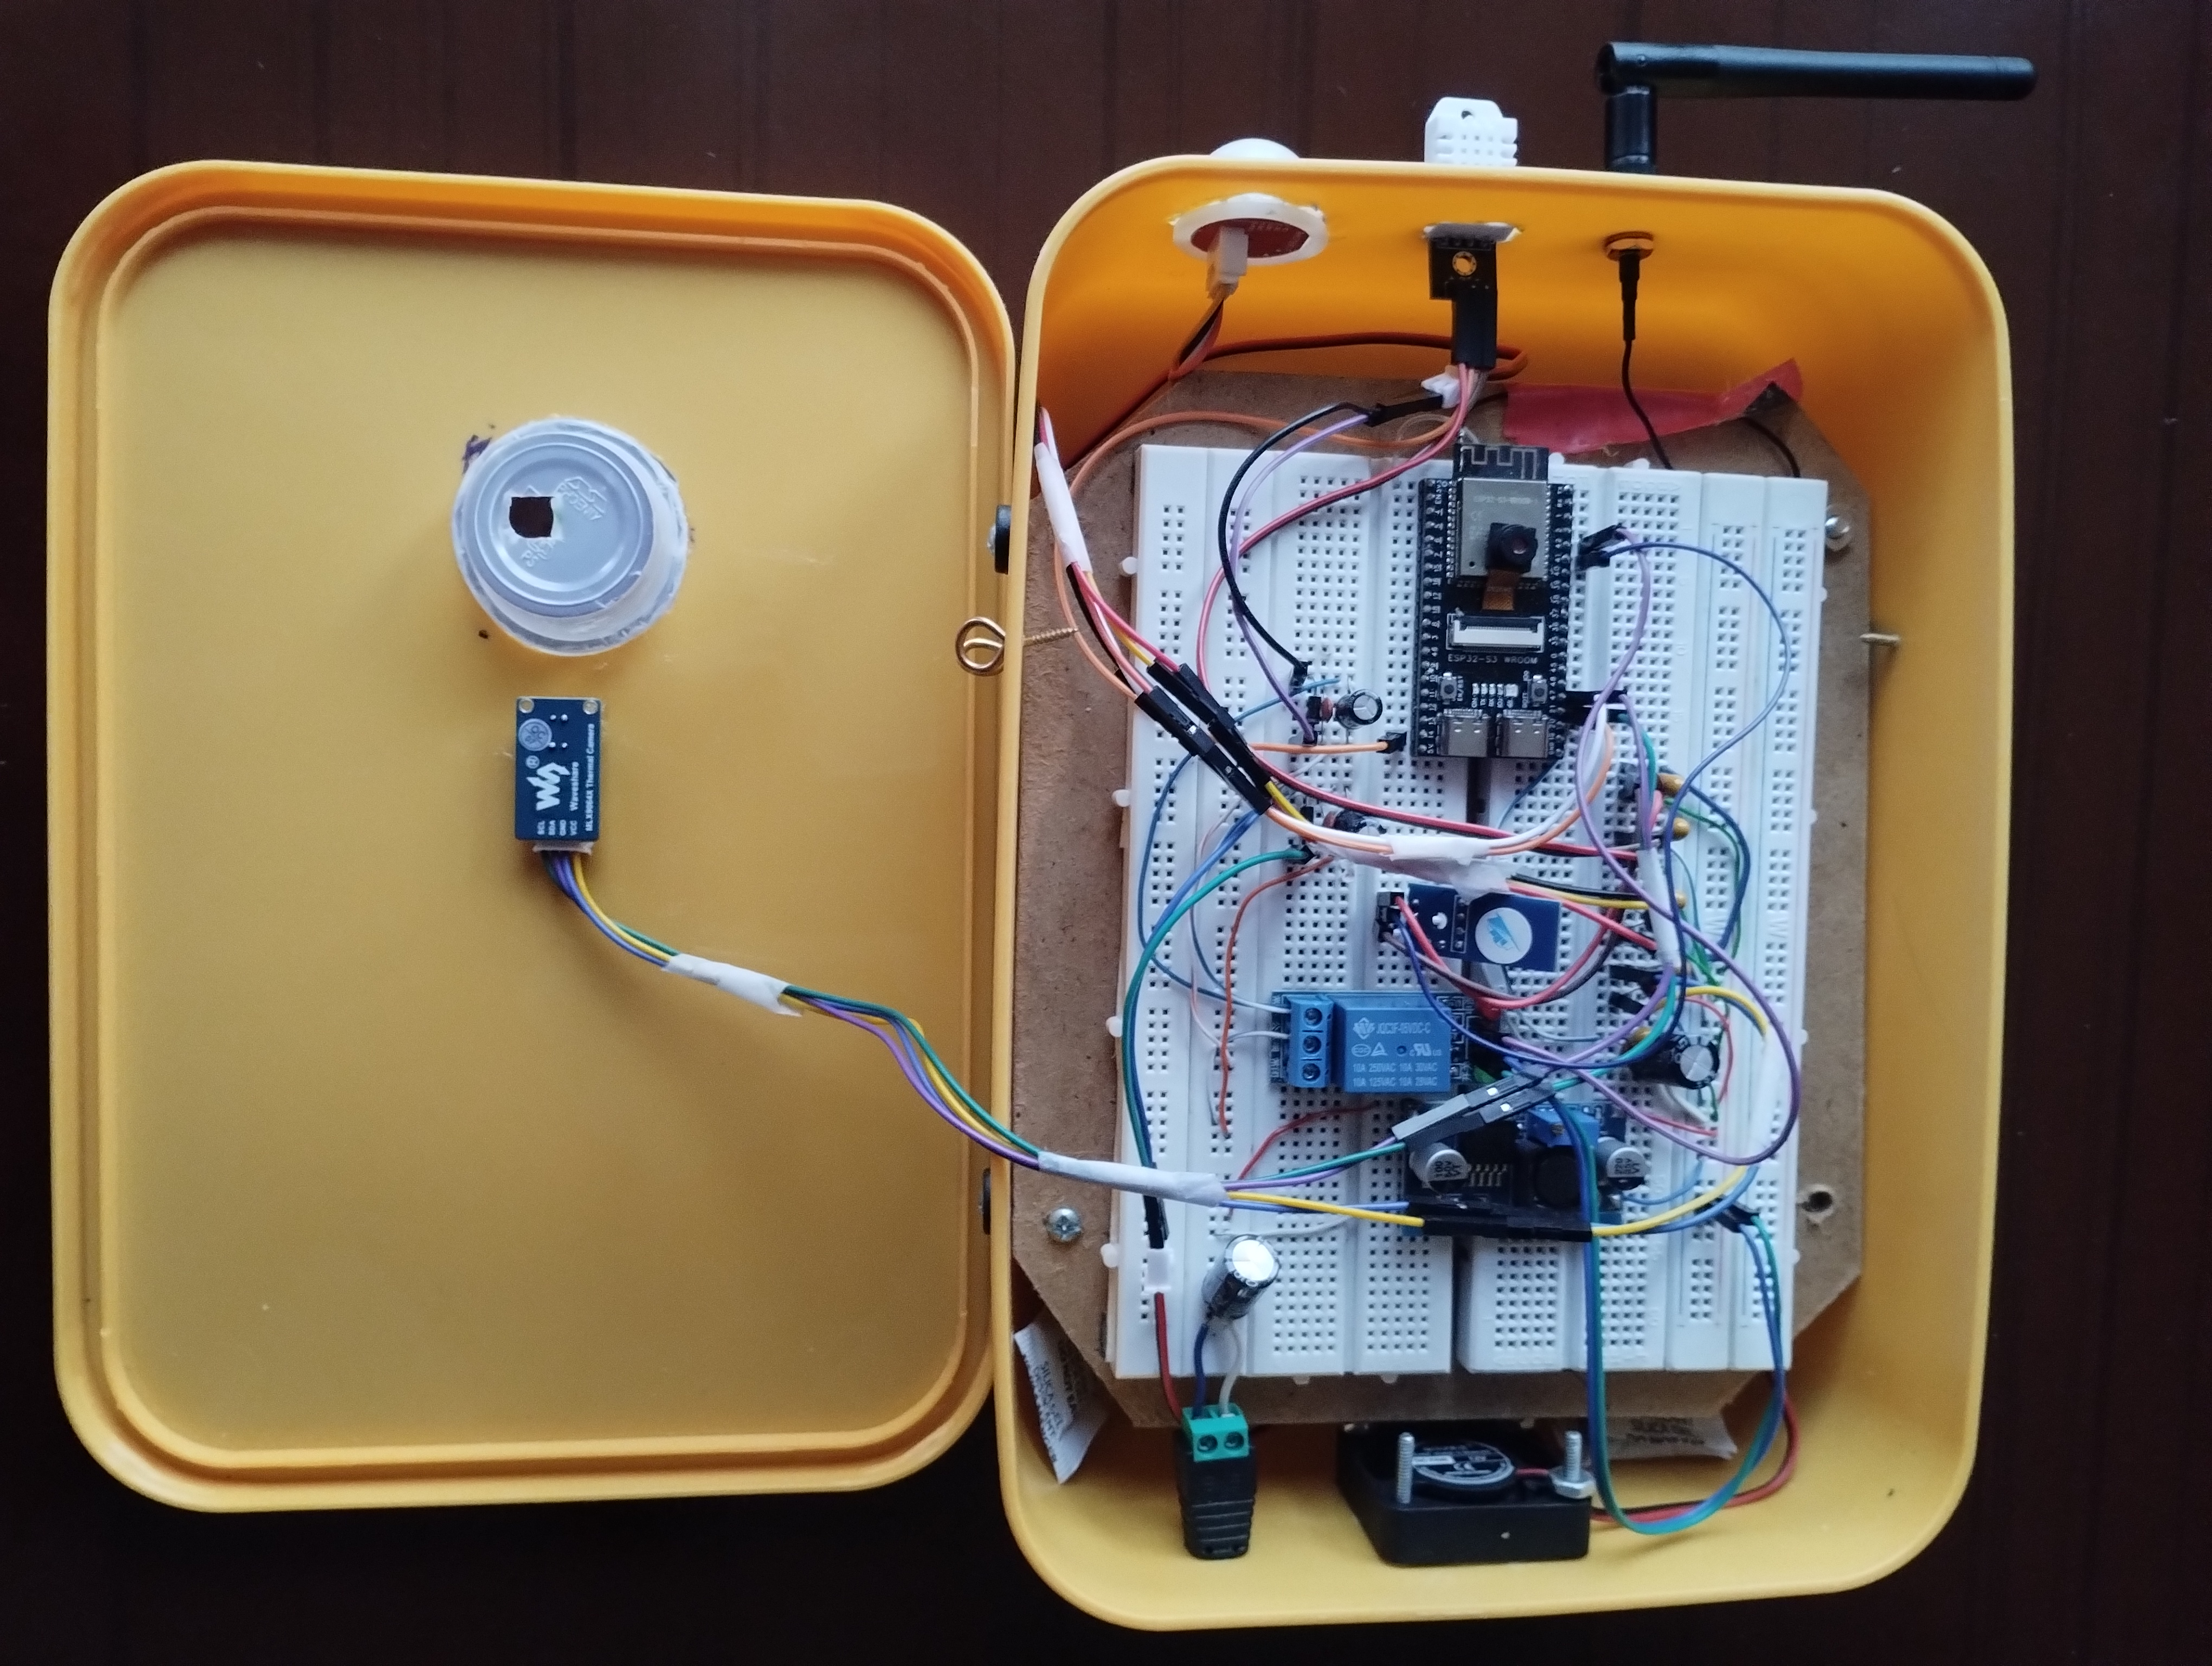
\includegraphics[width=0.6\textwidth]{img/prototipo1.jpg}
    \label{fig:prototipo_inicial}
\end{figure}

\begin{figure}[H]
    \centering
    \caption{Ensamblaje interno de los prototipos finales.}
    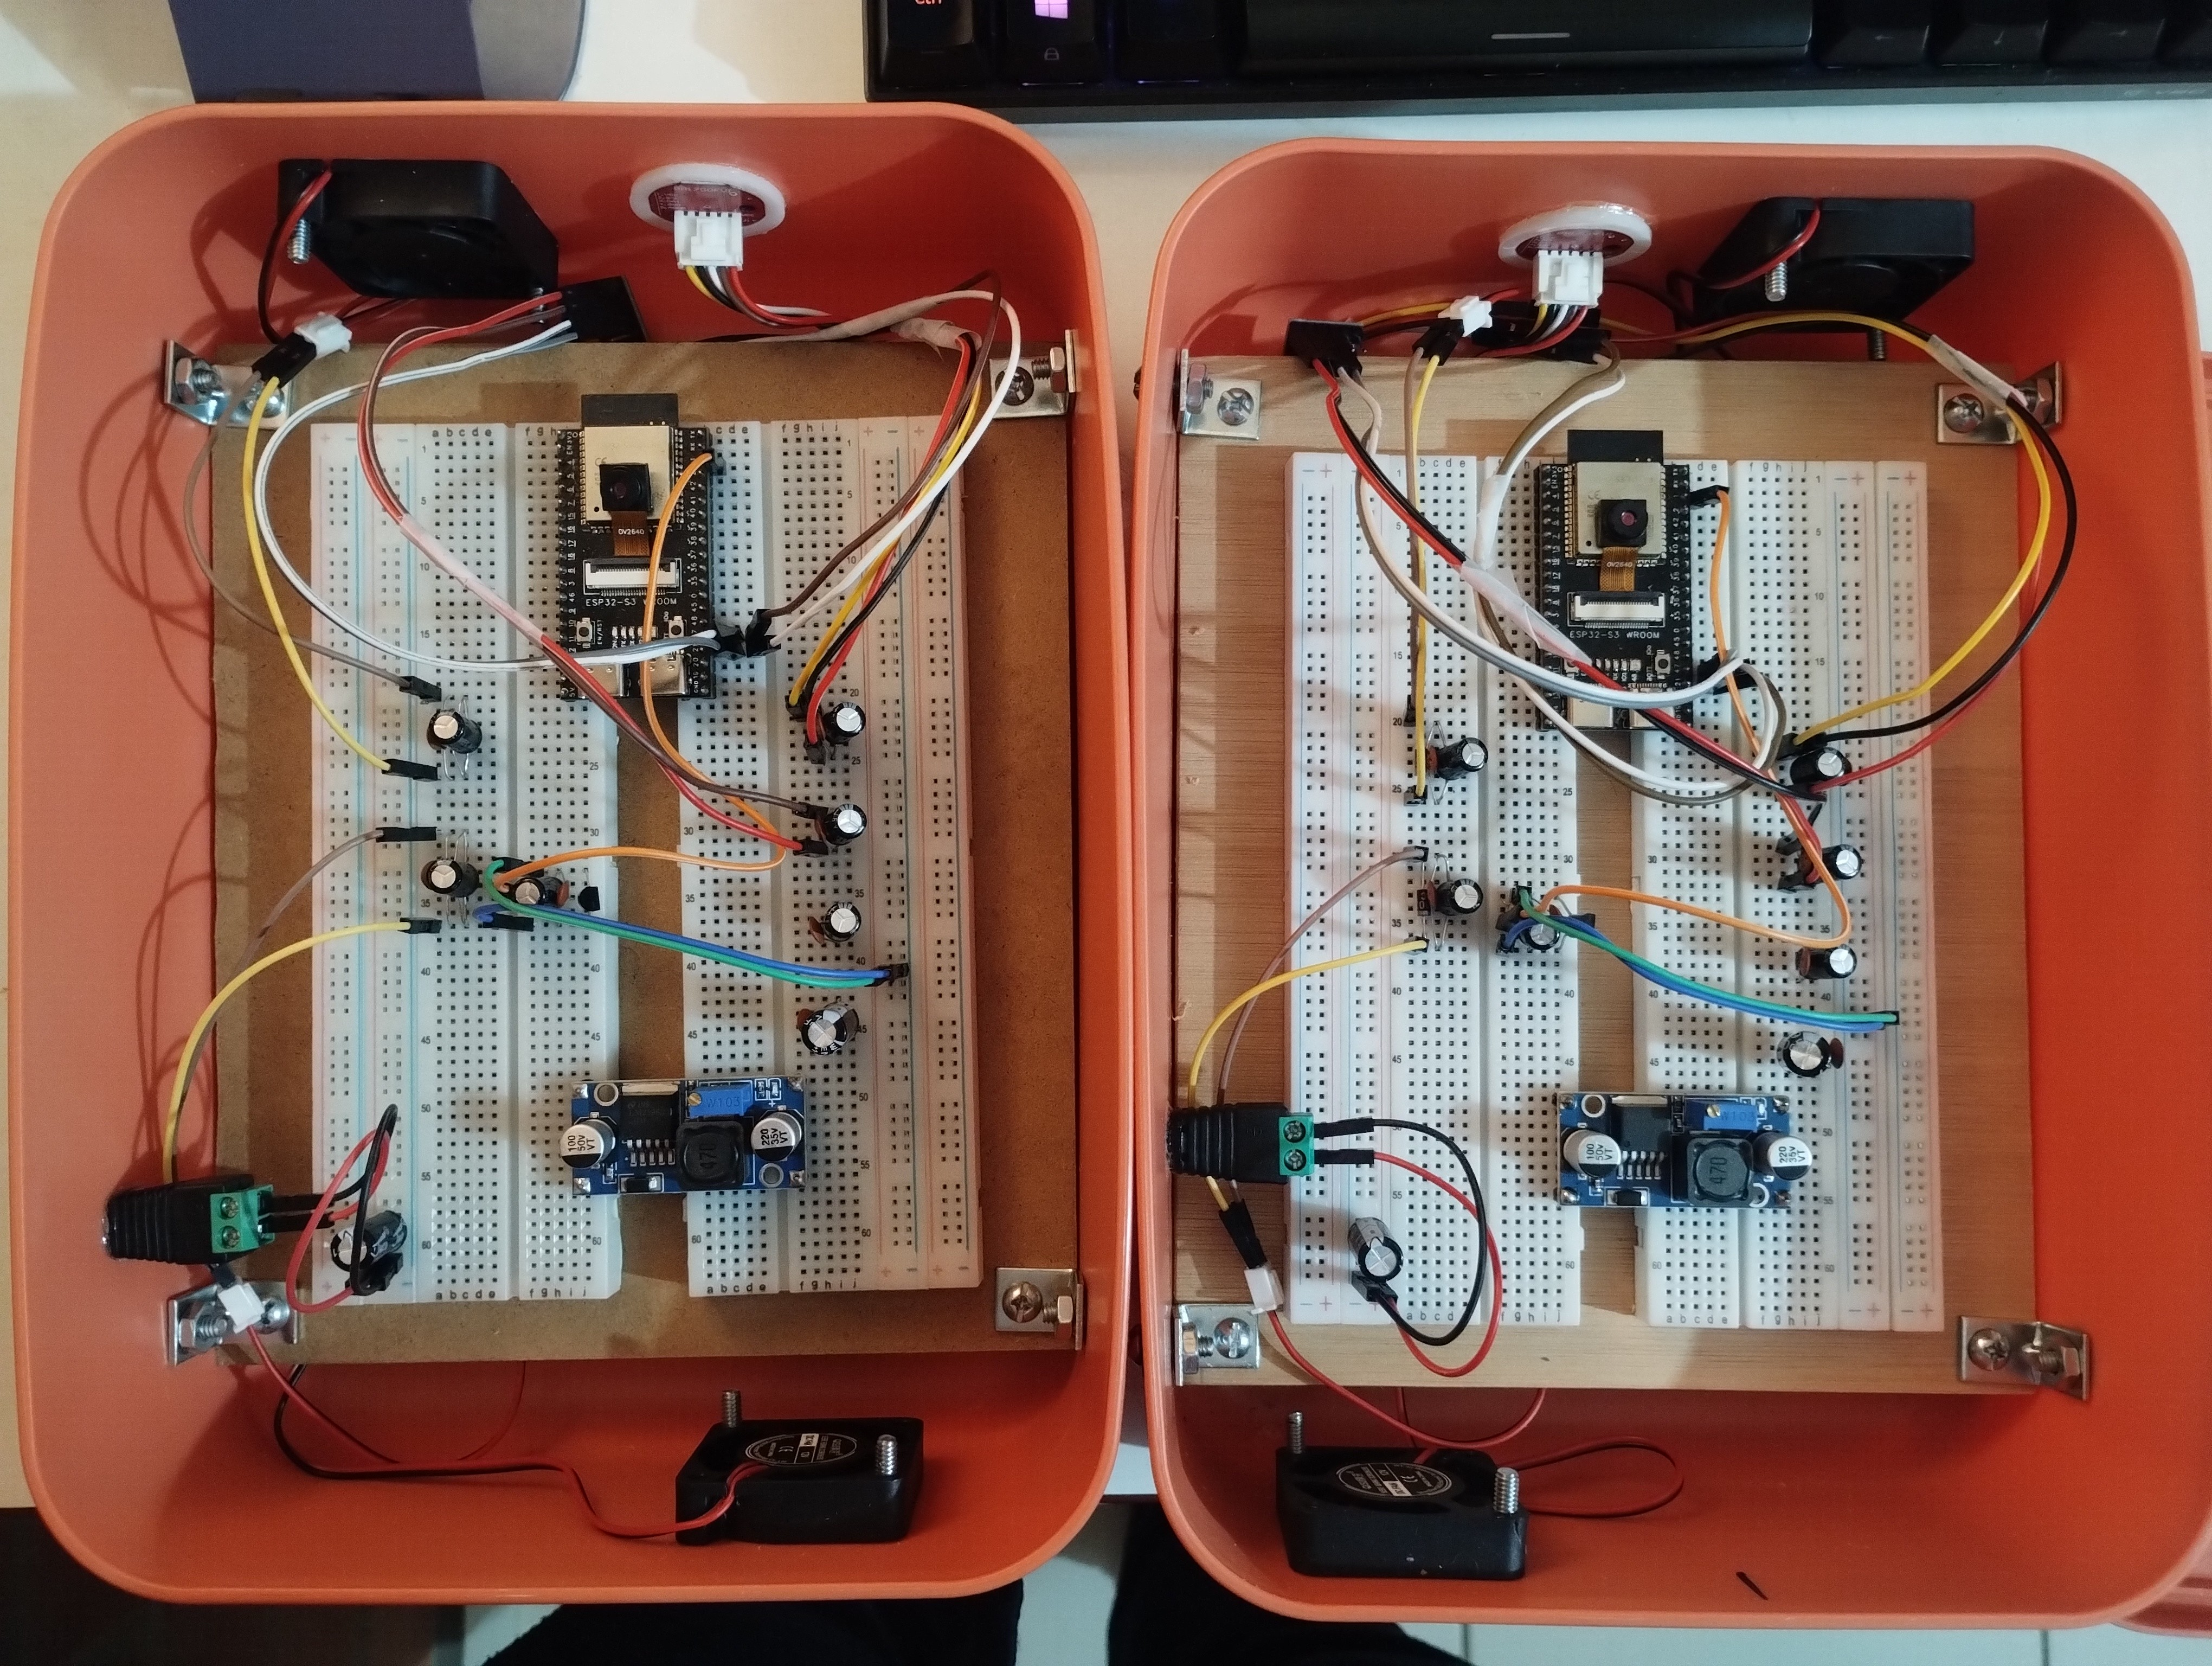
\includegraphics[width=0.8\textwidth]{img/prototipo2.jpg}
    
    \vspace{0.2cm}
    \begin{minipage}{0.8\textwidth}
    \small{\textit{Nota:} Ensamblaje utilizando protoboard.}
    \end{minipage}
    \label{fig:prototipo_final_1}
\end{figure}

\subsection{Desarrollo e integración del firmware}
\label{subsec:hardware_firmware}
El firmware para el microcontrolador ESP32-S3 se desarrolló utilizando el entorno de desarrollo integrado (IDE) Visual Studio Code con la extensión PlatformIO. PlatformIO facilita la gestión de proyectos embebidos, incluyendo la compilación, carga del firmware y manejo de dependencias \footnote{\url{https://platformio.org/}}. El framework de desarrollo empleado fue Arduino Core para ESP32 \footnote{\url{https://github.com/espressif/arduino-esp32}}, que proporciona un conjunto de librerías y funciones para interactuar con el hardware del microcontrolador de forma simplificada.

La arquitectura del firmware se organizó de manera modular, separando responsabilidades en diferentes librerías y archivos fuente, como se evidencia en la estructura del proyecto proporcionada. La carpeta `src` contiene la lógica principal de la aplicación (`main.cpp`), controladores de ciclo (`CycleController`) y tareas específicas para la adquisición de datos ambientales (`EnvironmentTasks`) y de imágenes (`ImageTasks`), así como la inicialización del sistema (`SystemInit`).

La carpeta `lib` alberga un conjunto de librerías personalizadas desarrolladas para este proyecto, encapsulando la interacción con cada sensor (`BH1750Sensor`, `BME280Sensor`, `MLX90640Sensor`, `OV2640Sensor`) y gestionando funcionalidades clave del sistema:
\begin{itemize}
    \item \textbf{Conectividad:} `WifiManager` para la gestión de la conexión a redes Wi-Fi.
    \item \textbf{Comunicación:} `API` y `MultipartDataSender` para el envío de datos a un servidor backend.
    \item \textbf{Interfaz web:} `WebPortal` para ofrecer una interfaz de configuración y monitoreo accesible vía navegador, utilizando `ESPAsyncWebServer`.
    \item \textbf{Almacenamiento:} `ConfigManager` para leer/escribir la configuración del dispositivo usando el sistema de archivos `LittleFS` \footnote{\url{https://github.com/littlefs-project/littlefs}}, y `SDManager` para interactuar con la tarjeta SD.
    \item \textbf{Gestión del tiempo:} `TimeManager` para obtener y gestionar la hora del sistema, posiblemente mediante NTP (Network Time Protocol).
    \item \textbf{Utilidades:} `LEDStatus` para controlar el LED RGB integrado, `ErrorLogger` para el registro de errores, y `EnvironmentDataJSON` para formatear los datos recolectados en JSON \footnote{\url{https://arduinojson.org/}}.
\end{itemize}

El desarrollo se apoyó en librerías de terceros gestionadas por PlatformIO, incluyendo `Adafruit MLX90640` \footnote{\url{https://github.com/adafruit/Adafruit_MLX90640}}, `BH1750` \footnote{\url{https://github.com/claws/BH1750}}, `Adafruit BME280 Library` \footnote{\url{https://github.com/adafruit/Adafruit_BME280_Library}}, `DallasTemperature` \footnote{\url{https://github.com/milesburton/Arduino-Temperature-Control-Library}} y `OneWire` \footnote{\url{https://github.com/PaulStoffregen/OneWire}} (sugiriendo pruebas con sensores DS18B20 no incluidos en el prototipo final), `ESPAsyncWebServer` \footnote{\url{https://github.com/me-no-dev/ESPAsyncWebServer}} con `AsyncTCP` \footnote{\url{https://github.com/me-no-dev/AsyncTCP}}, y `ArduinoJson` \footnote{\url{https://arduinojson.org/}} para la manipulación eficiente de datos JSON. La comunicación con los sensores I\textsuperscript{2}C (MLX90640, BME280, BH1750) se implementó utilizando la librería `Wire` estándar del framework Arduino \footnote{\url{https://www.arduino.cc/reference/en/language/functions/communication/wire/}}.

El flujo principal del firmware, orquestado en `main.cpp` y `CycleController`, involucra la inicialización de los componentes (`SystemInit`), la conexión a Wi-Fi, la sincronización horaria, y la ejecución periódica de tareas para leer los sensores ambientales y térmicos, capturar imágenes RGB, almacenar datos localmente (SD) y enviarlos al servidor backend a través de la API configurada. El portal web permite al usuario configurar parámetros como las credenciales Wi-Fi, la URL del servidor API y la frecuencia de muestreo.

\section{Metodología de caracterización y validación}
\label{sec:hardware_metodologia}
Para establecer la viabilidad y fiabilidad del prototipo como instrumento de medición en aplicaciones agrícolas, se diseñó e implementó una metodología de caracterización y validación experimental. Este proceso es indispensable para cuantificar la precisión del sistema y corregir posibles derivas instrumentales, un aspecto crítico al trabajar con sensores de bajo costo que son inherentemente más sensibles a las condiciones ambientales y al desgaste \shortcite{Jiao2022, Yun2023}. La metodología se estructuró en la definición de un sistema de referencia trazable y la ejecución de procedimientos experimentales específicos en entornos controlados.

\subsection{Sistema de referencia utilizado}
\label{subsec:hardware_sistema_referencia}
Se estableció un sistema de referencia para realizar las pruebas de calibración y evaluación de precisión del sensor térmico MLX90640. Este sistema permitió generar y medir temperaturas conocidas y estables que sirvieron como patrón de comparación para las lecturas del prototipo. Los componentes del sistema de referencia fueron (ver Figuras \ref{fig:cuerpo_gris} y \ref{fig:controlador_pid}):
\begin{itemize}
    \item \textbf{Cuerpo gris de emisividad conocida:} Se construyó un cuerpo gris utilizando una lámina de aluminio de $10 \times 15 \times 1$ cm, pintada con una capa de pintura negra mate resistente a altas temperaturas. Esta configuración asegura una emisividad alta y conocida, estimada en 0.96, lo cual es fundamental para mediciones termográficas precisas. Este cuerpo gris actuó como el objetivo cuya temperatura superficial sería medida por los prototipos. Para calentarlo de manera controlada, se colocó sobre una estufa eléctrica de resistencia.
    \item \textbf{Controlador de temperatura PID:} Se empleó un controlador de temperatura Proporcional-Integral-Derivativo (PID), modelo REX-C100 (RKC Instrument), para mantener la temperatura del cuerpo gris en un valor estable y predefinido durante las pruebas de calibración. El controlador ajustaba la potencia suministrada a la estufa eléctrica basándose en la retroalimentación de temperatura. Durante las pruebas con referencia estable, se configuraron temperaturas objetivo (SV - Set Value) de $170^{\circ}$C y $190^{\circ}$C.
    \item \textbf{Termocupla tipo K:} Para obtener la medición de referencia de la temperatura superficial del cuerpo gris con alta precisión, se utilizó una termocupla tipo K conectada directamente al controlador PID. Las termocuplas de este tipo ofrecen una precisión del orden de $\pm0.3^{\circ}$C en el rango de trabajo \shortcite{Acorsi2020}, sirviendo como el valor "verdadero" contra el cual se compararon las mediciones del sensor MLX90640. La punta de la termocupla se fijó en contacto directo con la superficie pintada del cuerpo gris.
\end{itemize}

% Figura Cuerpo Gris
\begin{figure}[H]
    \centering
    \caption{Cuerpo gris sobre estufa eléctrica.}
    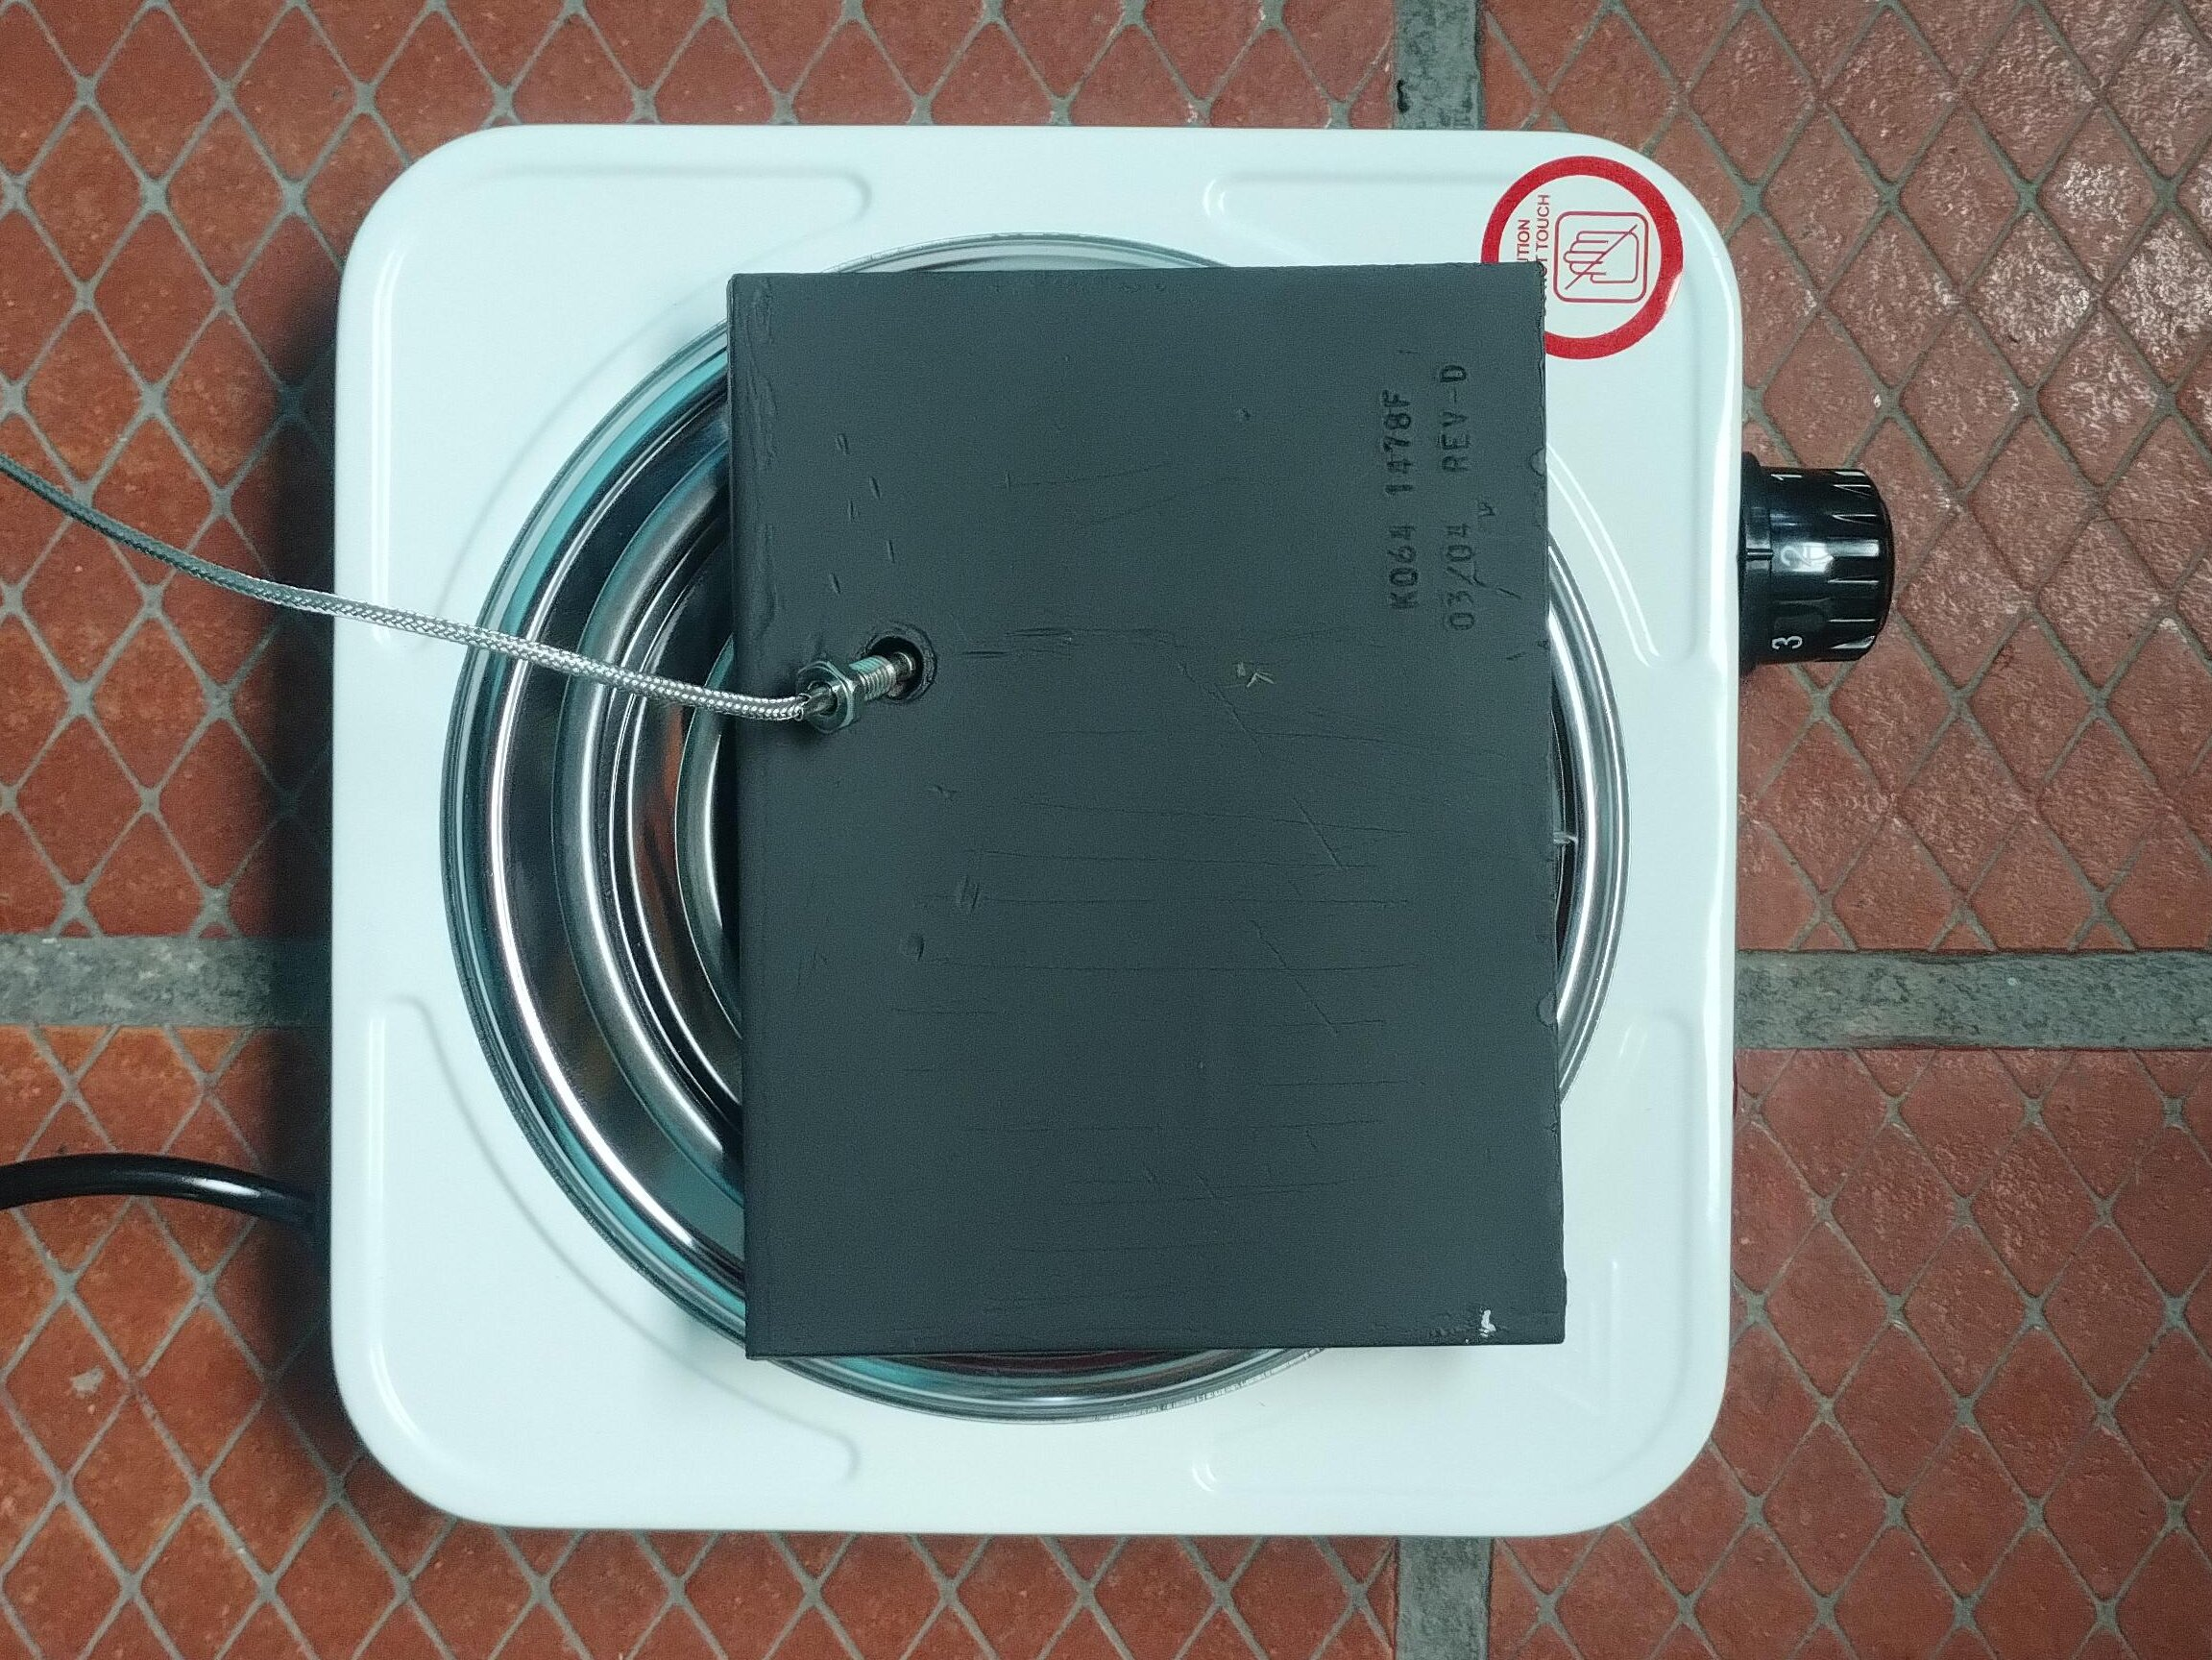
\includegraphics[width=0.7\textwidth]{img/cuerpogris.jpg}
    \vspace{0.2cm}
    \begin{minipage}{0.7\textwidth}
    \small{\textit{Nota:} Lámina de aluminio pintada de negro mate con termocupla tipo K insertada para medición de temperatura de referencia.}
    \end{minipage}
    \label{fig:cuerpo_gris}
\end{figure}

% Figura Controlador PID
\begin{figure}[H]
    \centering
    \caption{Controlador de temperatura PID REX-C100.}
    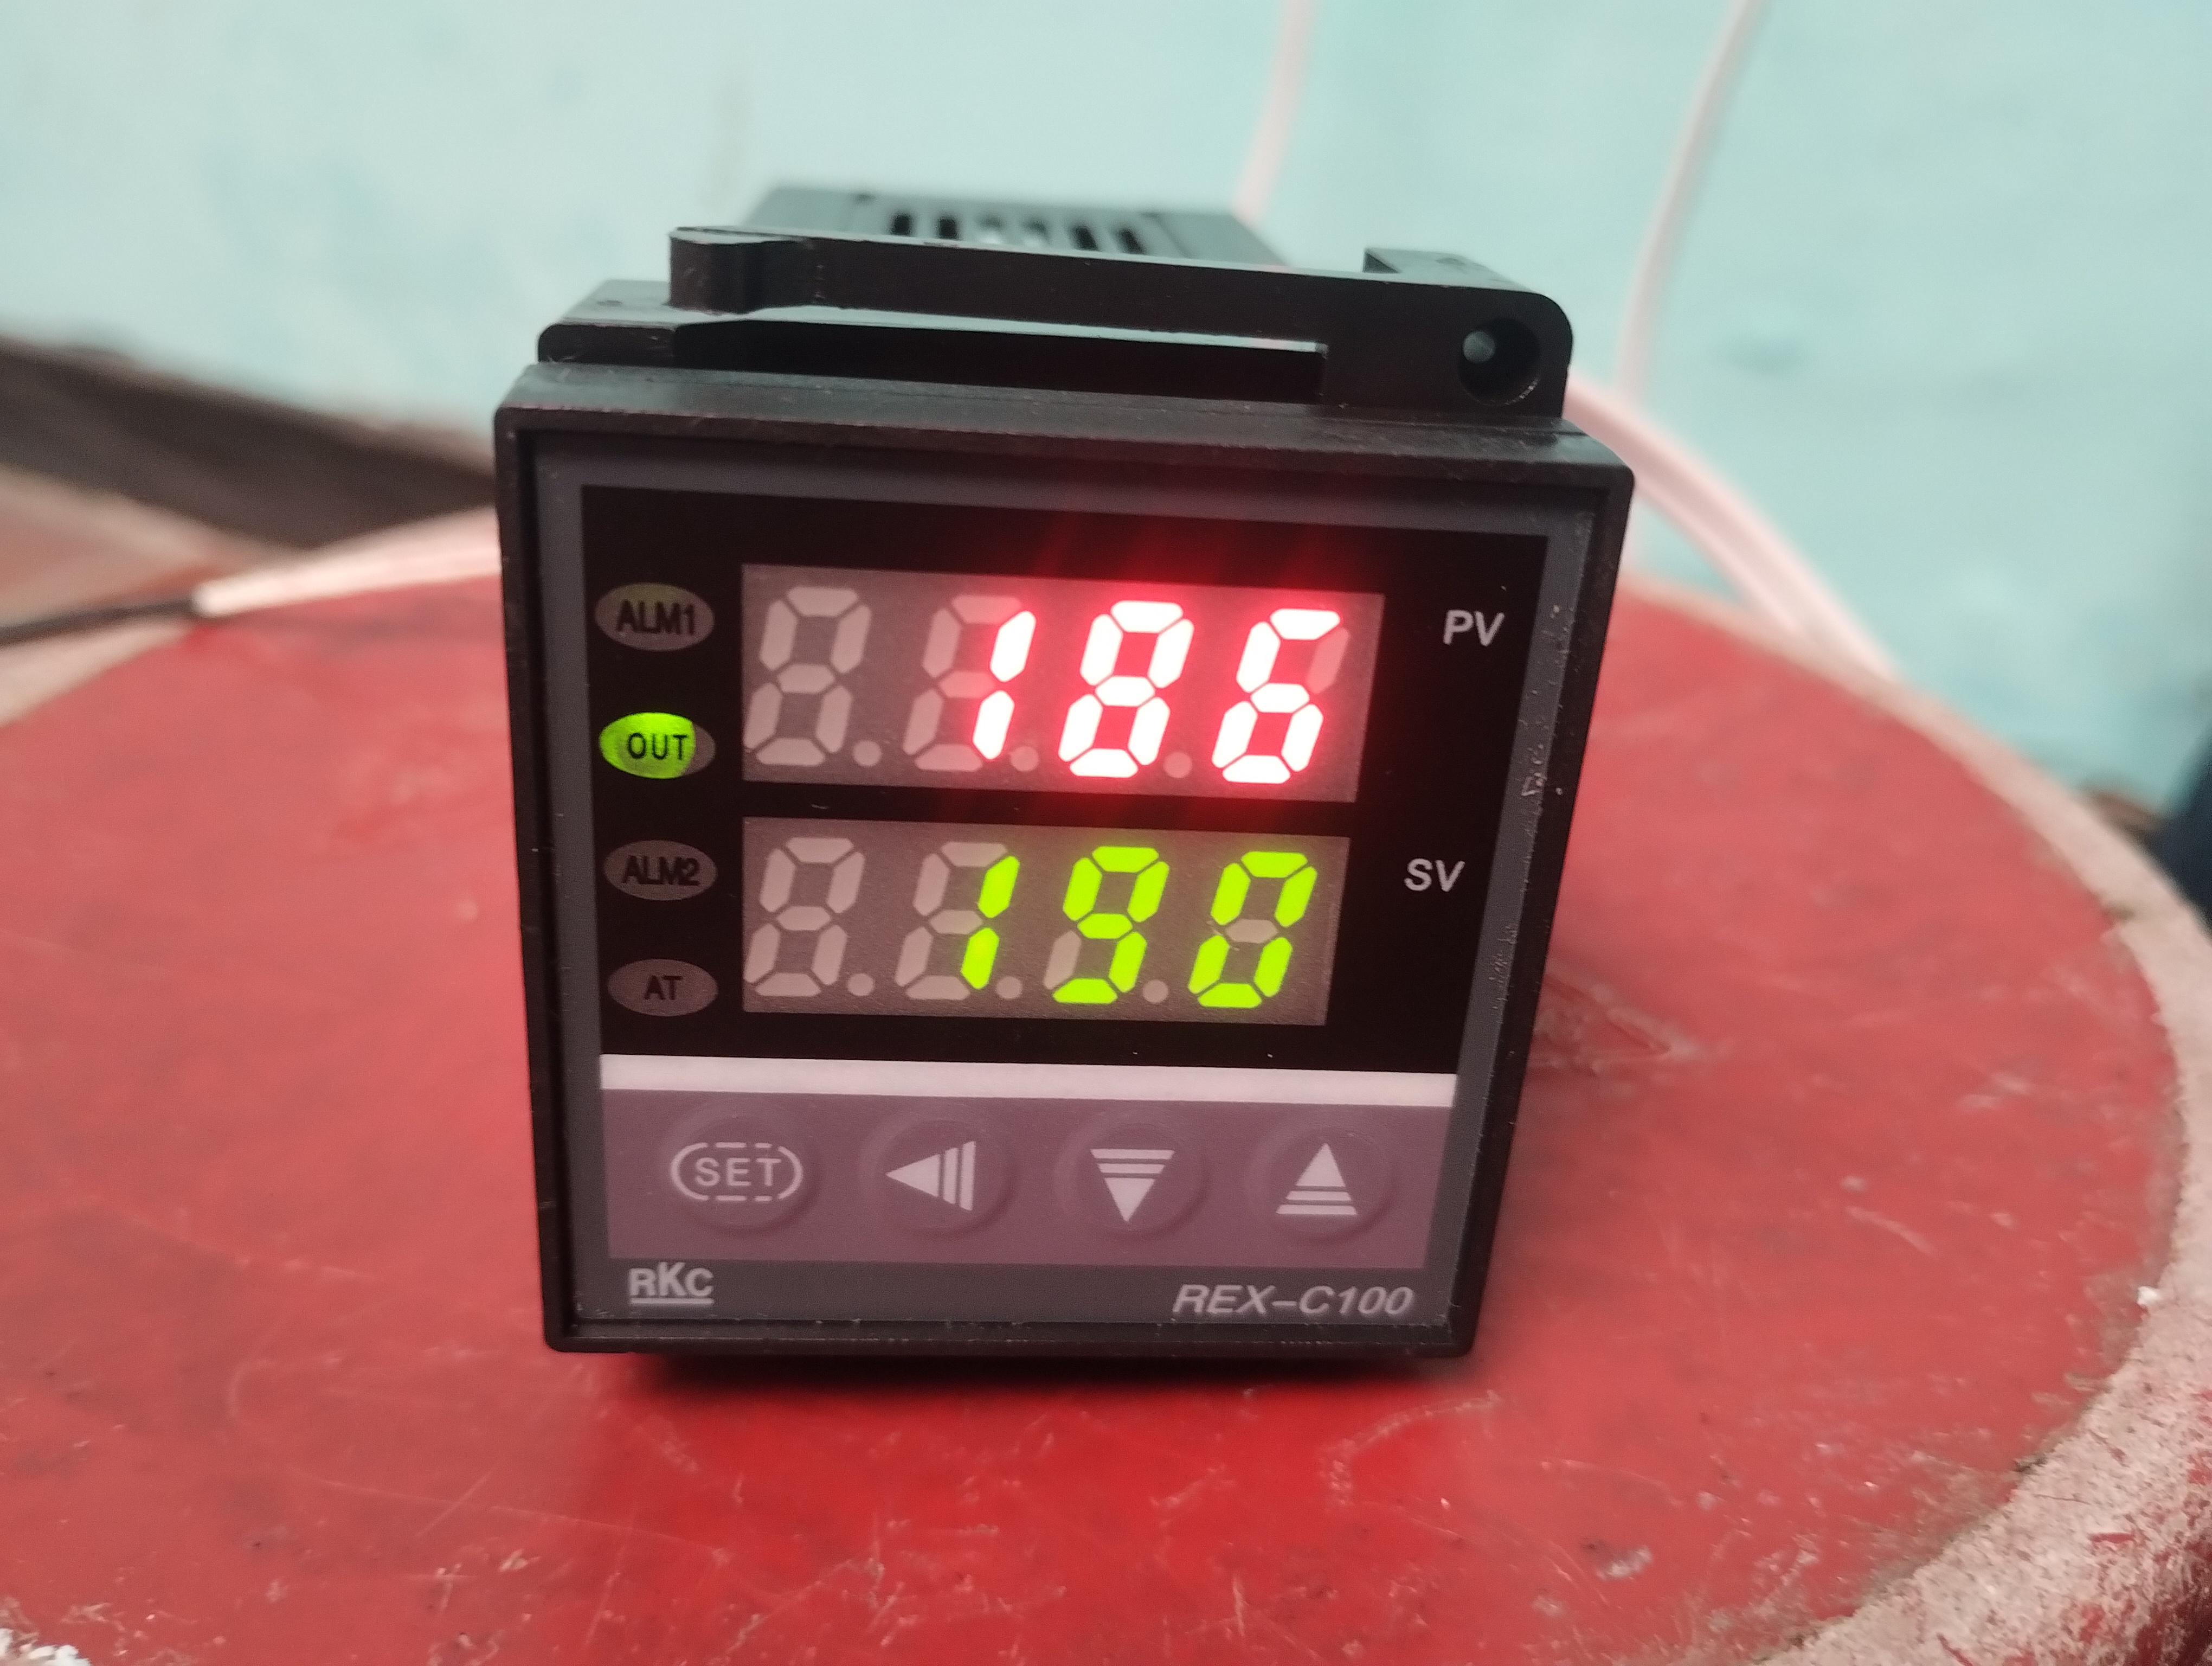
\includegraphics[width=0.5\textwidth]{img/pid.jpg}
    \vspace{0.2cm}
    \begin{minipage}{0.5\textwidth}
    \small{\textit{Nota:} Utilizado para estabilizar la temperatura del cuerpo gris. Muestra la temperatura medida (PV) y la temperatura objetivo (SV).}
    \end{minipage}
    \label{fig:controlador_pid}
\end{figure}

\subsection{Procedimientos experimentales}
\label{subsec:hardware_procedimientos}
Se ejecutaron dos tipos principales de pruebas experimentales: pruebas de calibración cuantitativa y una prueba de contraste térmico. Todas las pruebas se realizaron en entornos controlados para minimizar la interferencia de variables externas como corrientes de aire o fluctuaciones bruscas de la temperatura ambiente. Los entornos utilizados fueron un microinvernadero (condiciones cercanas a la aplicación final) y una habitación cerrada sin ventilación.

\textbf{Pruebas de calibración:} El objetivo principal fue evaluar la precisión y estabilidad de los sensores térmicos MLX90640 bajo diferentes condiciones ambientales y de temperatura objetivo. Se utilizó el sistema de referencia (cuerpo gris calentado y controlado por PID) como fuente de temperatura estable y conocida. Se realizaron cuatro configuraciones de prueba distintas:
\begin{enumerate}
    \item \textit{Prueba en espacio controlado con referencia inestable:} Se evaluó la respuesta inicial de los sensores a una fuente de calor menos controlada (aproximadamente $190^{\circ}$C) durante el día en una habitación cerrada. Esto permitió observar la dinámica inicial y posibles derivas rápidas.
    \item \textit{Prueba en invernadero con referencia estable (diurna):} Se analizó la precisión en el microinvernadero durante el día, usando una temperatura de referencia estable de $170^{\circ}$C. Esta prueba buscaba simular condiciones de operación diurnas, incluyendo la posible influencia de la radiación solar indirecta en el entorno del invernadero.
    \item \textit{Prueba en invernadero con referencia estable (nocturna):} Se repitió la prueba anterior durante la noche, manteniendo la referencia estable a $170^{\circ}$C, para evaluar el desempeño en ausencia de radiación solar y con temperaturas ambientales potencialmente diferentes.
    \item \textit{Prueba en espacio controlado con referencia estable:} Se realizaron mediciones con una temperatura de referencia estable de aproximadamente $190^{\circ}$C durante la noche en la habitación cerrada. Esta prueba permitió confirmar el comportamiento observado a alta temperatura sin las posibles perturbaciones ambientales presentes en el microinvernadero.
\end{enumerate}

\subsection{Resultados de la caracterización térmica}
\label{subsec:hardware_resultados_termico}

En la Figura \ref{fig:calibracion1} se presentan los resultados de las pruebas de calibración térmica utilizando el cuerpo gris estabilizado con el controlador PID a diferentes temperaturas de referencia ($180^{\circ}$C, $45^{\circ}$C y $25^{\circ}$C). El ensayo comparó simultáneamente el desempeño de las cámaras nuevas (Prototipos 1 y 2) frente a la cámara previamente utilizada (Prototipo 3), abarcando mediciones diurnas (tarde) y nocturnas. El análisis de las series temporales demuestra que los sensores nuevos presentan una alta precisión y estabilidad, manteniendo una correlación muy estrecha con la temperatura de referencia. En contraste, la cámara usada (Waveshare) exhibe un nivel sustancial de ruido de alta frecuencia y una alta descalibración (\textit{drift}), registrando valores erráticos y alejados de los reales, independientemente del régimen de temperatura o la hora del día. Esto confirma que el desgaste físico continuo degrada la fiabilidad del sensor térmico MLX90640.

\begin{figure}[H]
    \centering
    \caption{Pruebas térmicas de calibración.}
    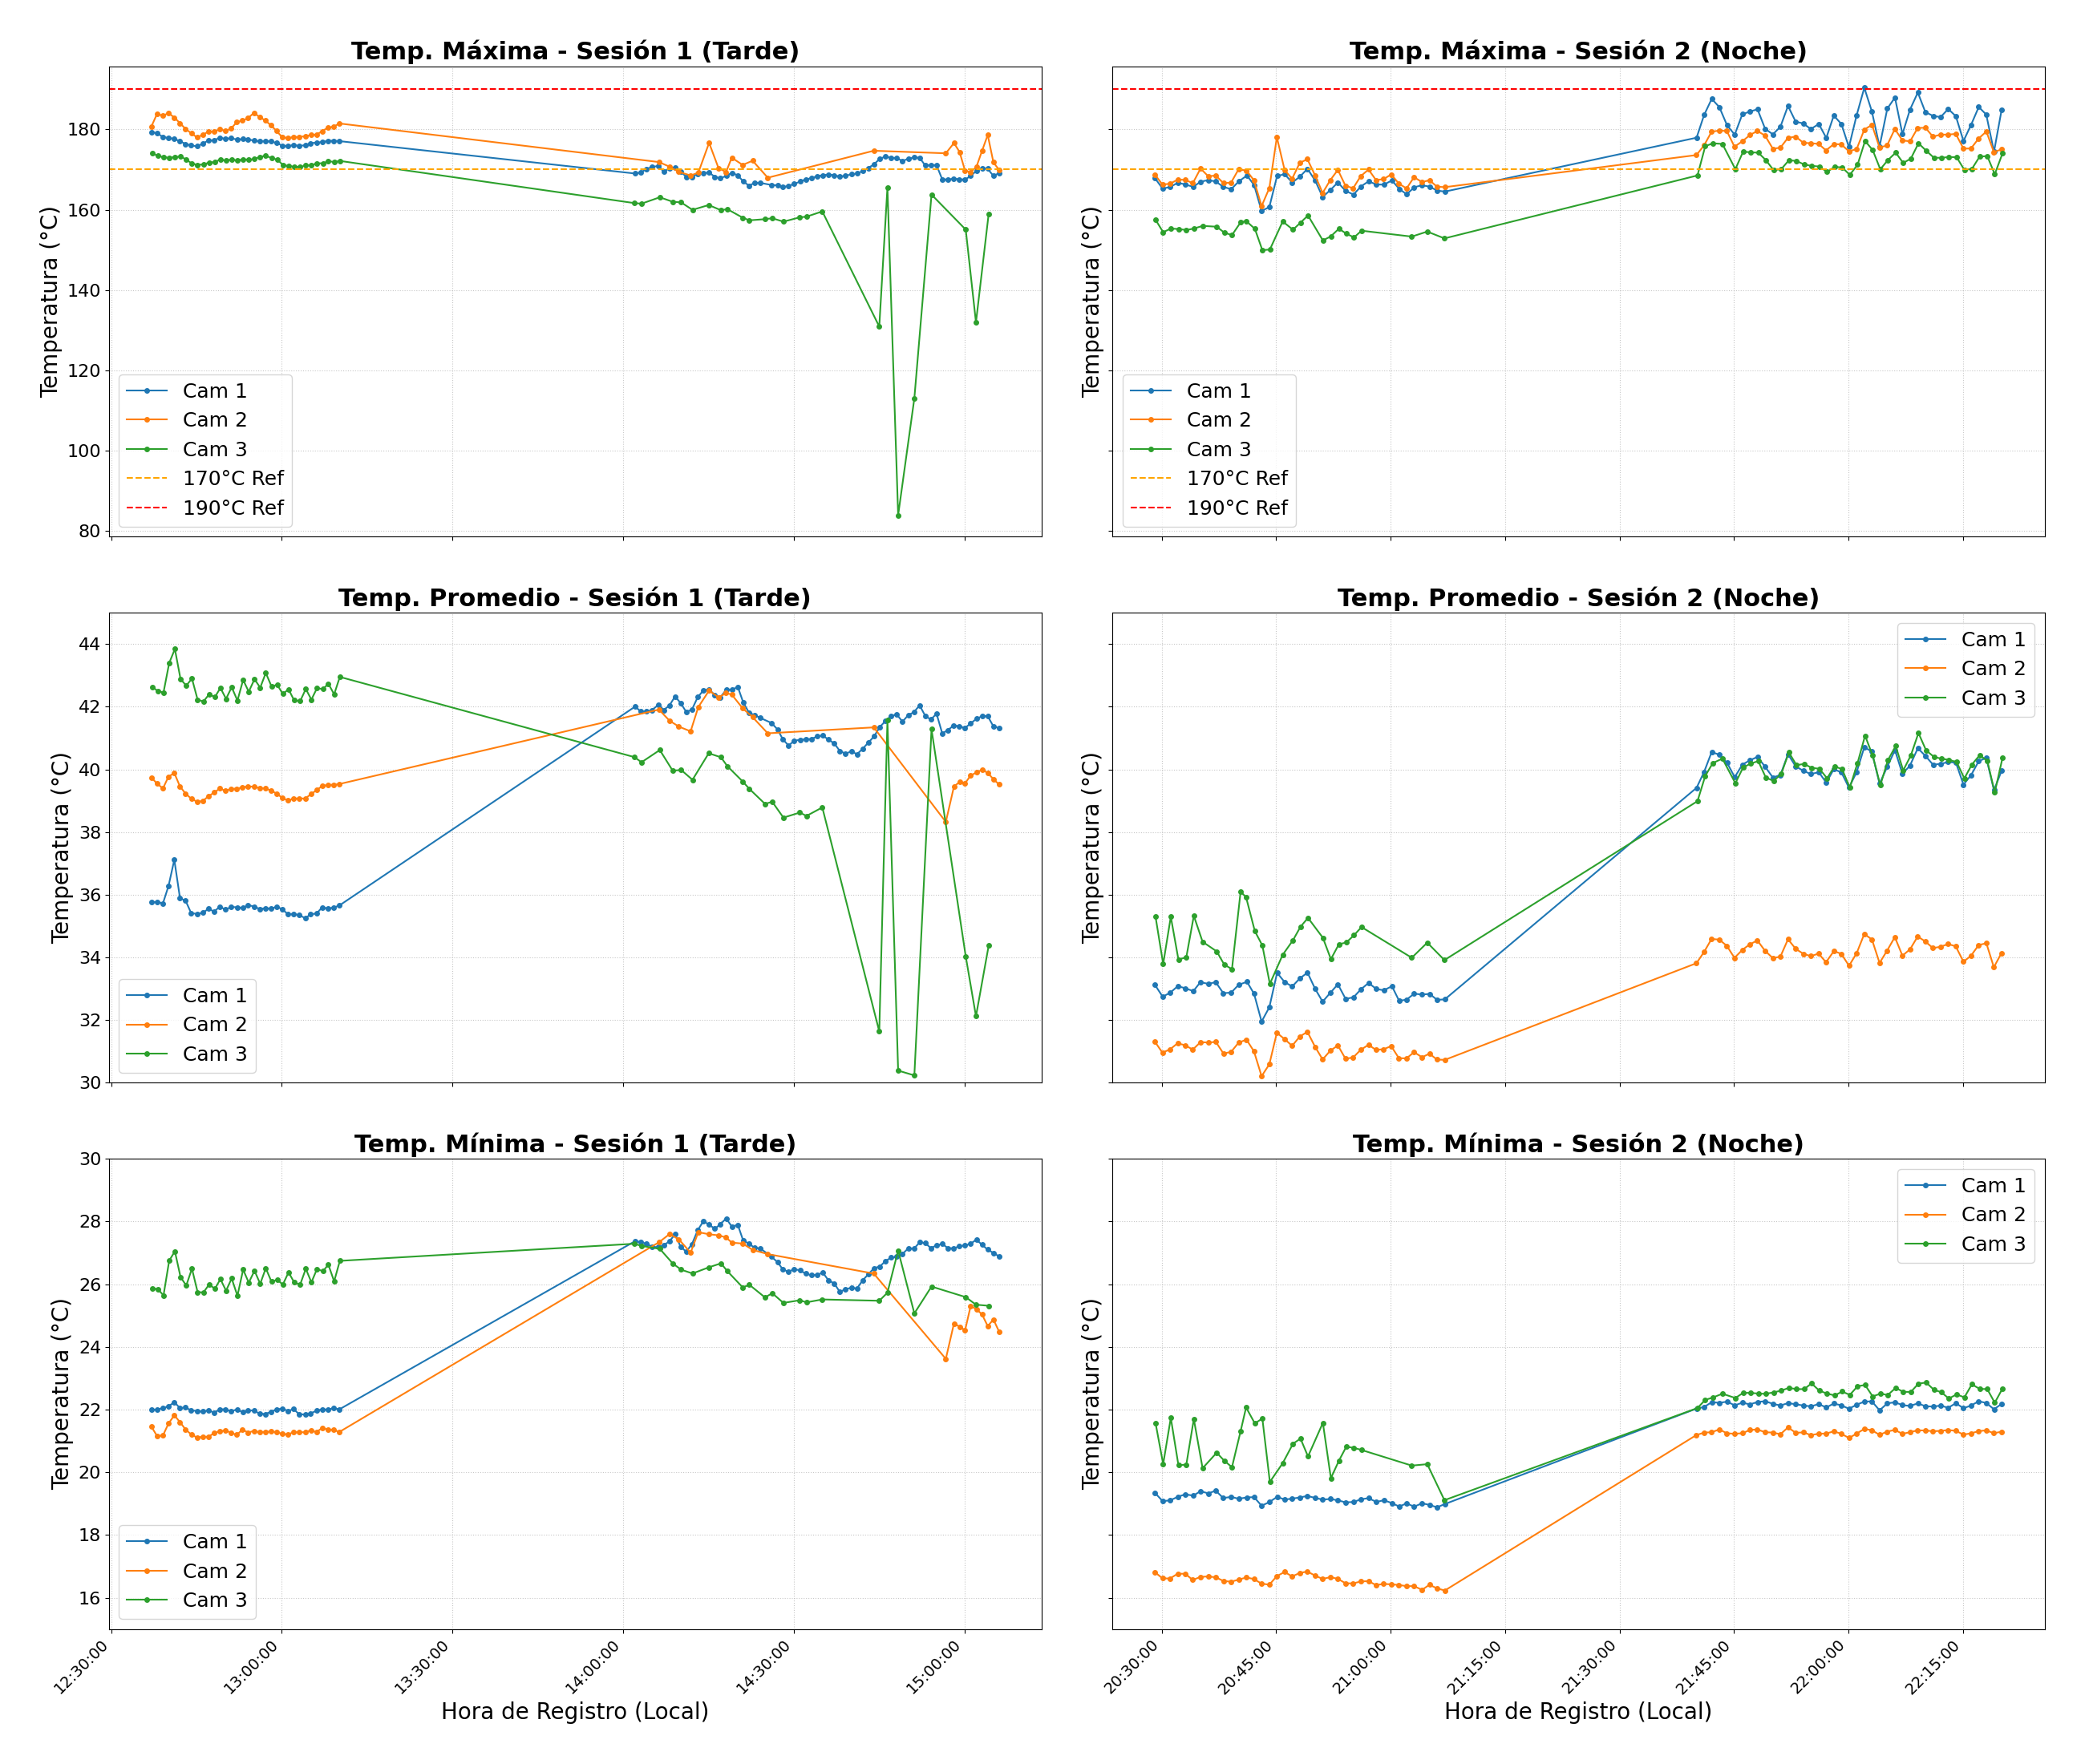
\includegraphics[width=\textwidth]{img/calibracion1.png}
    
    \vspace{0.2cm}
    \begin{minipage}{\textwidth}
    \small{\textit{Nota:} Comparación entre dos cámaras nuevas y una usada (tarde y noche) a temperaturas de referencia de 180$^\circ$C, 45$^\circ$C y 25$^\circ$C usando el cuerpo gris.}
    \end{minipage}
    \label{fig:calibracion1}
\end{figure}

Para complementar lo anterior, la Figura \ref{fig:calibracion2} ilustra una prueba de verificación exclusiva entre las dos cámaras nuevas en un espectro más amplio de temperaturas ($20^{\circ}$C, $30^{\circ}$C, $170^{\circ}$C y $190^{\circ}$C) ejecutada en una única sesión prolongada. Los resultados reafirman la consistencia de los dispositivos nuevos, mostrando una diferencia de precisión prácticamente nula entre ambos, validando la fiabilidad de estos sensores para construir una red de monitoreo homogénea, siempre y cuando se encuentren en óptimas condiciones físicas.

\begin{figure}[H]
    \centering
    \caption{Prueba de verificación térmica posterior.}
    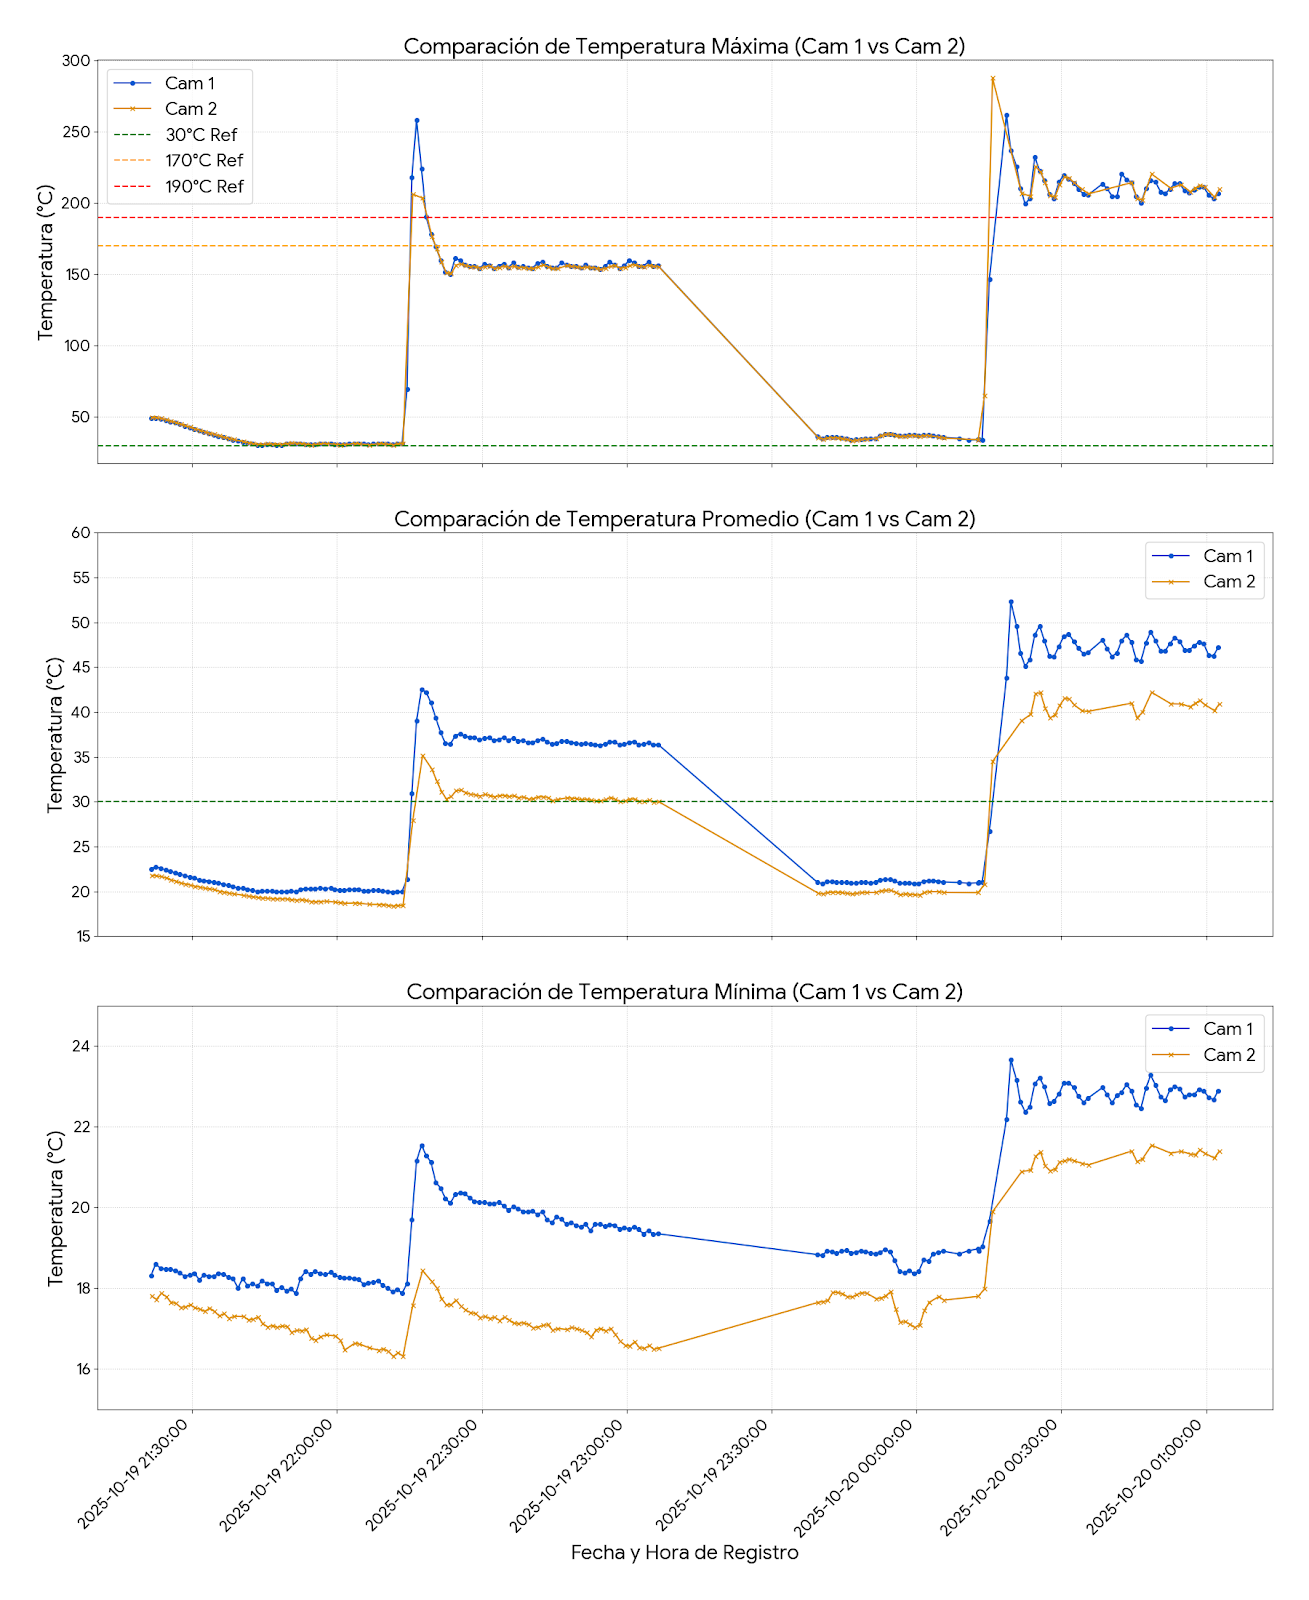
\includegraphics[width=\textwidth]{img/calibracion2.png}
    
    \vspace{0.2cm}
    \begin{minipage}{\textwidth}
    \small{\textit{Nota:} Pruebas realizadas exclusivamente entre las cámaras nuevas en rangos de 20$^\circ$C, 30$^\circ$C, 170$^\circ$C y 190$^\circ$C.}
    \end{minipage}
    \label{fig:calibracion2}
\end{figure}

Adicionalmente, se ejecutó una prueba de contraste térmico (Figura \ref{fig:contraste_termico}) exponiendo los sensores simultáneamente a un elemento frío (hielo en agua) y un elemento caliente (agua recién hervida a 2550m s. n. m.). Esta prueba dinámica evidenció un comportamiento anómalo y no lineal en la cámara usada: presenta una descalibración aguda y ruido severo al registrar temperaturas bajas y medias, pero paradójicamente logra censar las temperaturas altas con un comportamiento medianamente aceptable. Esto sugiere que el desgaste térmico no afecta por igual a todos los fotodiodos infrarrojos de la matriz del sensor o que el rango dinámico de amplificación del componente dañado falla desproporcionadamente en los rangos inferiores. La caracterización térmica demostró cuantitativamente que el sensor MLX90640 previamente utilizado presentaba una degradación significativa, haciéndolo inadecuado para futuras mediciones fiables.

\begin{figure}[H]
    \centering
    \caption{Prueba de contraste térmico extremo.}
    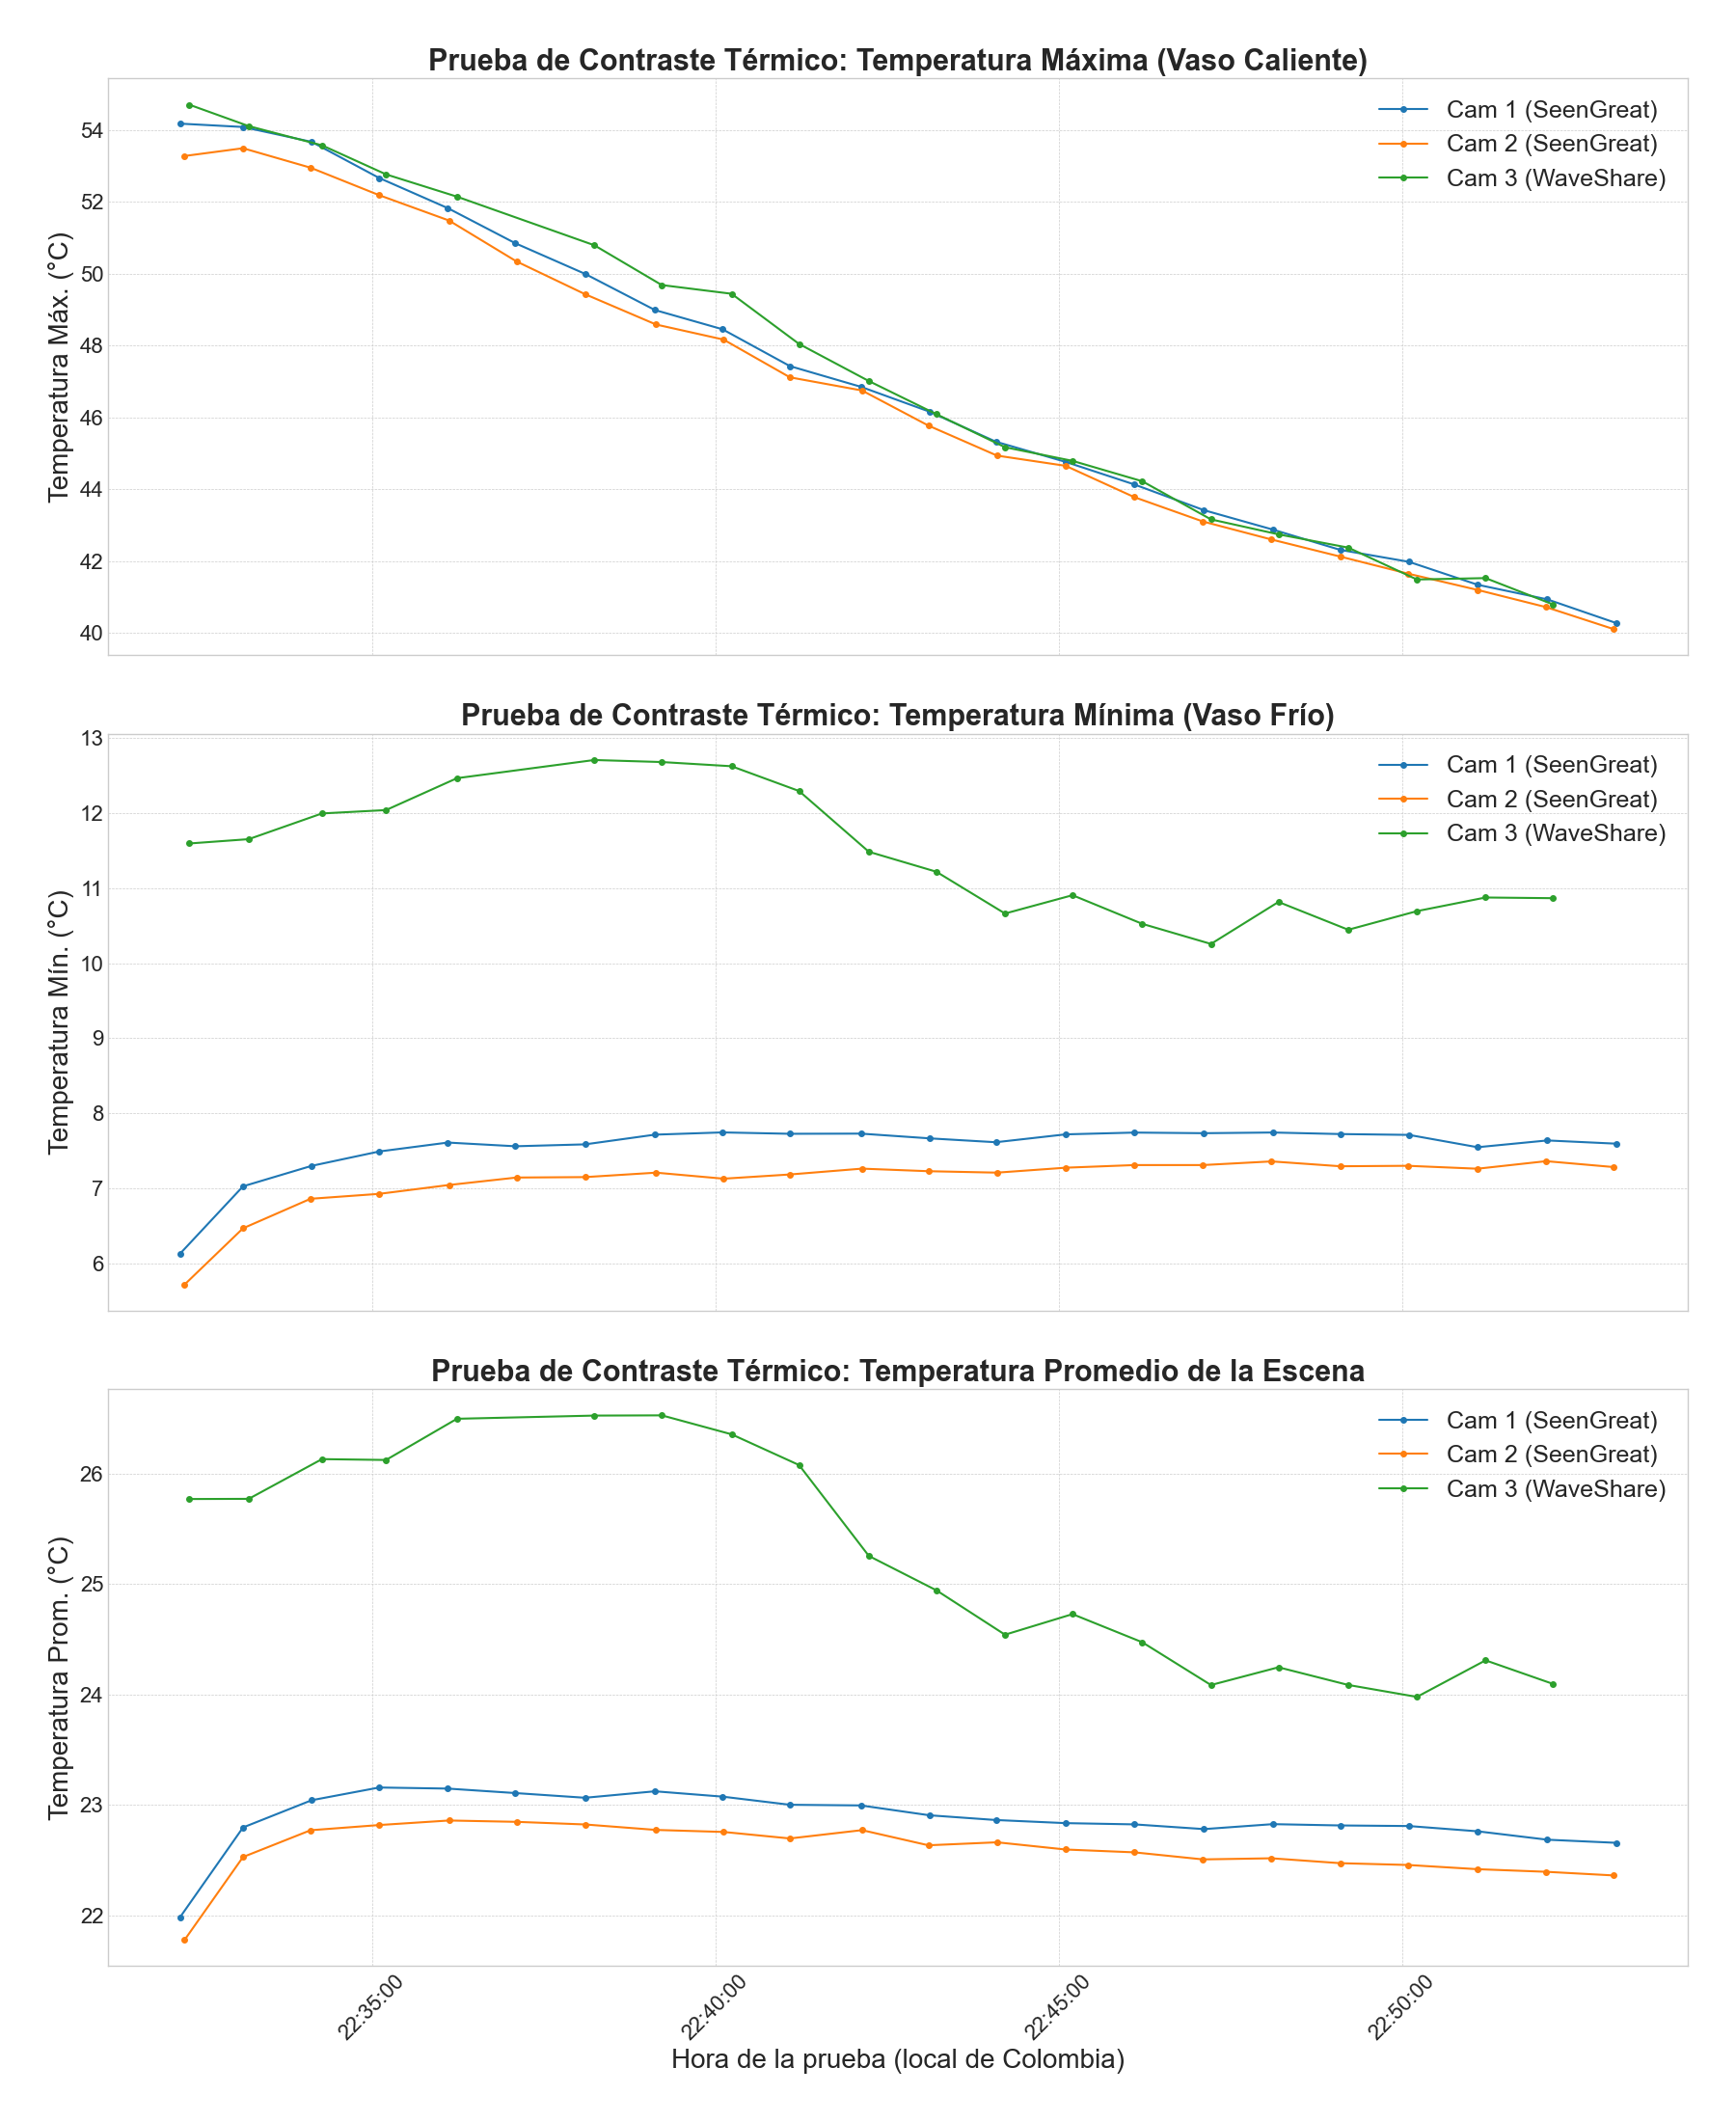
\includegraphics[width=\textwidth]{img/contraste_termico.png}
    
    \vspace{0.2cm}
    \begin{minipage}{\textwidth}
    \small{\textit{Nota:} Prueba de respuesta a gradientes severos frente a hielo y agua recién hervida.}
    \end{minipage}
    \label{fig:contraste_termico}
\end{figure}

\subsection{Análisis estadístico y evaluación de incertidumbre en la medición}

Para validar la fiabilidad de los datos recolectados por el sistema de captura, se realizó un análisis cuantitativo del desempeño térmico de las cámaras frente a temperaturas patrón. Para complementar el análisis gráfico previo, el objetivo principal de esta sección es cuantificar el estado de funcionamiento del sensor térmico usado (el cual estuvo operando y registrando datos de forma continua durante un periodo de 55 días) frente al comportamiento de los sensores completamente nuevos. Los cálculos estadísticos presentados a continuación se extrajeron exclusivamente de las pruebas de alto estrés térmico (170$^{\circ}$C y 190$^{\circ}$C), ya que estas condiciones permiten evidenciar claramente la descalibración (\textit{drift}), el ruido y la pérdida de precisión en el componente desgastado, proporcionando un buen punto de contraste analítico.

A partir de los datos registrados en las pruebas de calibración térmica, se extrajeron la media, la mediana, la desviación estándar y el error medio. Estos resultados se consolidan en la Tabla \ref{tab:indicadores_estadisticos}.

\begin{table}[H]
    \centering
    \caption{Resumen de indicadores estadísticos por prueba y dispositivo.}
    \resizebox{\textwidth}{!}{\begin{tabular}{llccccc}
        \toprule
        \textbf{Prueba} & \textbf{Dispositivo} & \textbf{Muestras ($n$)} & \textbf{Media ($^\circ$C)} & \textbf{Mediana ($^\circ$C)} & \textbf{Desv. Est.} & \textbf{Error Medio ($^\circ$C)} \\
        \midrule
        1 (Ref: 190 $^\circ$C) & Cam 1 & 34 & 177,08 & 177,08 & 0,85 & -12,92 \\
        1 (Ref: 190 $^\circ$C) & Cam 2 & 34 & 180,54 & 180,19 & 1,96 & -9,46 \\
        1 (Ref: 190 $^\circ$C) & Cam 3 & 34 & 172,17 & 172,21 & 0,88 & -17,83 \\
        2 (Ref: 170 $^\circ$C) & Cam 1 & 64 & 169,14 & 168,90 & 1,97 & -0,86 \\
        2 (Ref: 170 $^\circ$C) & Cam 2 & 23 & 171,95 & 171,16 & 2,90 & 1,95 \\
        2 (Ref: 170 $^\circ$C) & Cam 3 & 25 & 152,72 & 159,00 & 18,76 & -17,28 \\
        3 (Ref: 170 $^\circ$C) & Cam 1 & 39 & 165,98 & 166,15 & 2,00 & -4,02 \\
        3 (Ref: 170 $^\circ$C) & Cam 2 & 39 & 167,84 & 167,44 & 2,71 & -2,16 \\
        3 (Ref: 170 $^\circ$C) & Cam 3 & 28 & 154,73 & 154,97 & 2,01 & -15,27 \\
        4 (Ref: 190 $^\circ$C) & Cam 1 & 41 & 182,51 & 183,37 & 3,67 & -7,49 \\
        4 (Ref: 190 $^\circ$C) & Cam 2 & 41 & 177,34 & 177,07 & 2,01 & -12,66 \\
        4 (Ref: 190 $^\circ$C) & Cam 3 & 40 & 172,41 & 172,37 & 2,35 & -17,59 \\
        \bottomrule
    \end{tabular}}
    \label{tab:indicadores_estadisticos}
\end{table}

\textbf{Análisis de los indicadores:}
\begin{itemize}
    \item \textbf{Media y mediana:} La media representa la tendencia central del nivel de temperatura medido por el sistema, mientras que la mediana refleja el valor del percentil 50. La comparación de ambos permite identificar el impacto de lecturas atípicas (\textit{outliers}). Por ejemplo, en la Prueba 2 para la Cam 3, la diferencia de más de 6 $^\circ$C entre la media (152,72 $^\circ$C) y la mediana (159,00 $^\circ$C) evidencia perturbaciones transitorias severas que arrastran el promedio general, siendo la mediana un estimador más robusto del estado estacionario del sensor.
    \item \textbf{Desviación estándar:} Cuantifica la precisión (dispersión) de las lecturas. Valores bajos, como los 0,85 $^\circ$C en la Cam 1 (Prueba 1), demuestran una alta repetibilidad y estabilidad temporal en la medición. Por el contrario, desviaciones que superan los 18 $^\circ$C denotan inestabilidad térmica o fallos momentáneos en la adquisición.
    \item \textbf{Error medio:} Define la exactitud frente al patrón de referencia. Se observa una tendencia sistemática hacia valores negativos (alcanzando desfases de hasta -17,83 $^\circ$C), lo cual indica que los sensores registran sistemáticamente temperaturas inferiores a las del punto focal de calor.
\end{itemize}

\textbf{Análisis de Incertidumbre en la Medición:}

La discrepancia documentada en el error medio y las fluctuaciones evidenciadas por la desviación estándar requieren una caracterización de la incertidumbre. En el contexto de este hardware, la incertidumbre se deriva de tres fuentes principales:

\begin{enumerate}
    \item \textbf{Pérdidas y gradientes térmicos:} Es la causa primordial del error sistemático negativo. El acoplamiento térmico entre el objeto medido y la lente infrarroja sufre disipación al interactuar con la temperatura ambiente. Esto genera un microclima en la superficie del sensor que es marginalmente más frío que la fuente emisora real \shortcite{Yun2023}.
    \item \textbf{Ruido electromagnético y autocalentamiento:} Las variaciones transitorias de voltaje en el circuito impreso (PCB) y la interferencia en la transmisión de señales digitales/analógicas introducen dispersión aleatoria en la lectura de los píxeles térmicos.
    \item \textbf{Error de cuantización (ADC):} La conversión de la señal física a datos digitales introduce un truncamiento en la resolución, limitando la capacidad del sistema para reflejar variaciones térmicas sub-grado de forma continua.
\end{enumerate}

\textbf{Métodos de Contención y Mitigación:}

Para contener el impacto de estas fuentes de incertidumbre, se pueden emplear estrategias combinadas a nivel de hardware y software:

\begin{itemize}
    \item \textbf{Mitigación en firmware (filtro temporal):} Actualmente, el diseño del sistema integra un mecanismo de contención primario a nivel de firmware. La cámara procesa 6 imágenes térmicas en ventanas de 15 segundos y transmite un arreglo promediado al software. Este procedimiento actúa matemáticamente como un filtro paso bajo que atenúa la desviación estándar generada por el ruido aleatorio de alta frecuencia, entregando una matriz térmica mucho más estable.
    \item \textbf{Compensación algorítmica (software):} Dado que el error medio detectado es un sesgo sistemático y predecible a ciertos rangos (ej. desfases de aprox. -12 $^\circ$C al medir cerca de 190 $^\circ$C), es posible implementar una regresión lineal polinómica en el software. Dicho algoritmo aplicaría un \textit{offset} de compensación dinámico a los datos crudos antes de su visualización, corrigiendo la caída térmica.
    \item \textbf{Aislamiento físico (hardware):} De forma hipotética para futuras iteraciones del diseño, el uso de recubrimientos de baja conductividad térmica en la carcasa del sensor y mejoras en el blindaje del cableado de datos ayudarían a reducir las pérdidas por convección y el ruido electromagnético respectivamente.
\end{itemize}

\textbf{Consideraciones y Limitaciones para Futuras Iteraciones:}

El contraste entre el dispositivo usado y los nuevos evidencia que los sensores térmicos de bajo costo son altamente susceptibles a la descalibración en el corto plazo, siendo afectados significativamente por las condiciones ambientales y el desgaste propio de la operación continua (como se observó tras los 55 días de uso ininterrumpido) \shortcite{Jiao2022, Yun2023}.

A partir de estas observaciones, se establece como un lineamiento metodológico obligatorio para futuras iteraciones que el protocolo de calibración se acote al contexto real de la aplicación. Es decir, las pruebas de precisión y exactitud deben realizarse estrictamente en los rangos de temperatura operativos acordes al sujeto de medición. Para el caso de monitoreo de estrés en plantas, la calibración debe garantizar la fiabilidad del sensor dentro de una ventana térmica de entre 10 $^\circ$C y 50 $^\circ$C, evitando extrapolar márgenes de error de pruebas realizadas a altas temperaturas que no reflejan el escenario de medición final.

\subsection{Resultados de la caracterización ambiental y de luminosidad}
\label{subsec:hardware_resultados_amb}

En relación con las variables ambientales, la Figura \ref{fig:comparacion_ambiental} presenta el contraste entre los sensores ambientales BME280 (nuevos, instalados en los Prototipos 1 y 2) y el sensor DHT22 (usado, Prototipo 3). El análisis longitudinal de las mediciones de temperatura y humedad relativa corrobora que ambos sensores BME280 ofrecen lecturas virtualmente idénticas a lo largo del tiempo, demostrando la alta repetibilidad de la tecnología microelectromecánica. Por su parte, el sensor DHT22 manifiesta signos inequívocos de \textit{drift} o descalibración temporal, evidenciado por oscilaciones erráticas y sesgos frente a los sensores nuevos bajo las mismas condiciones ambientales.

\begin{figure}[H]
    \centering
    \caption{Comparación de sensores ambientales.}
    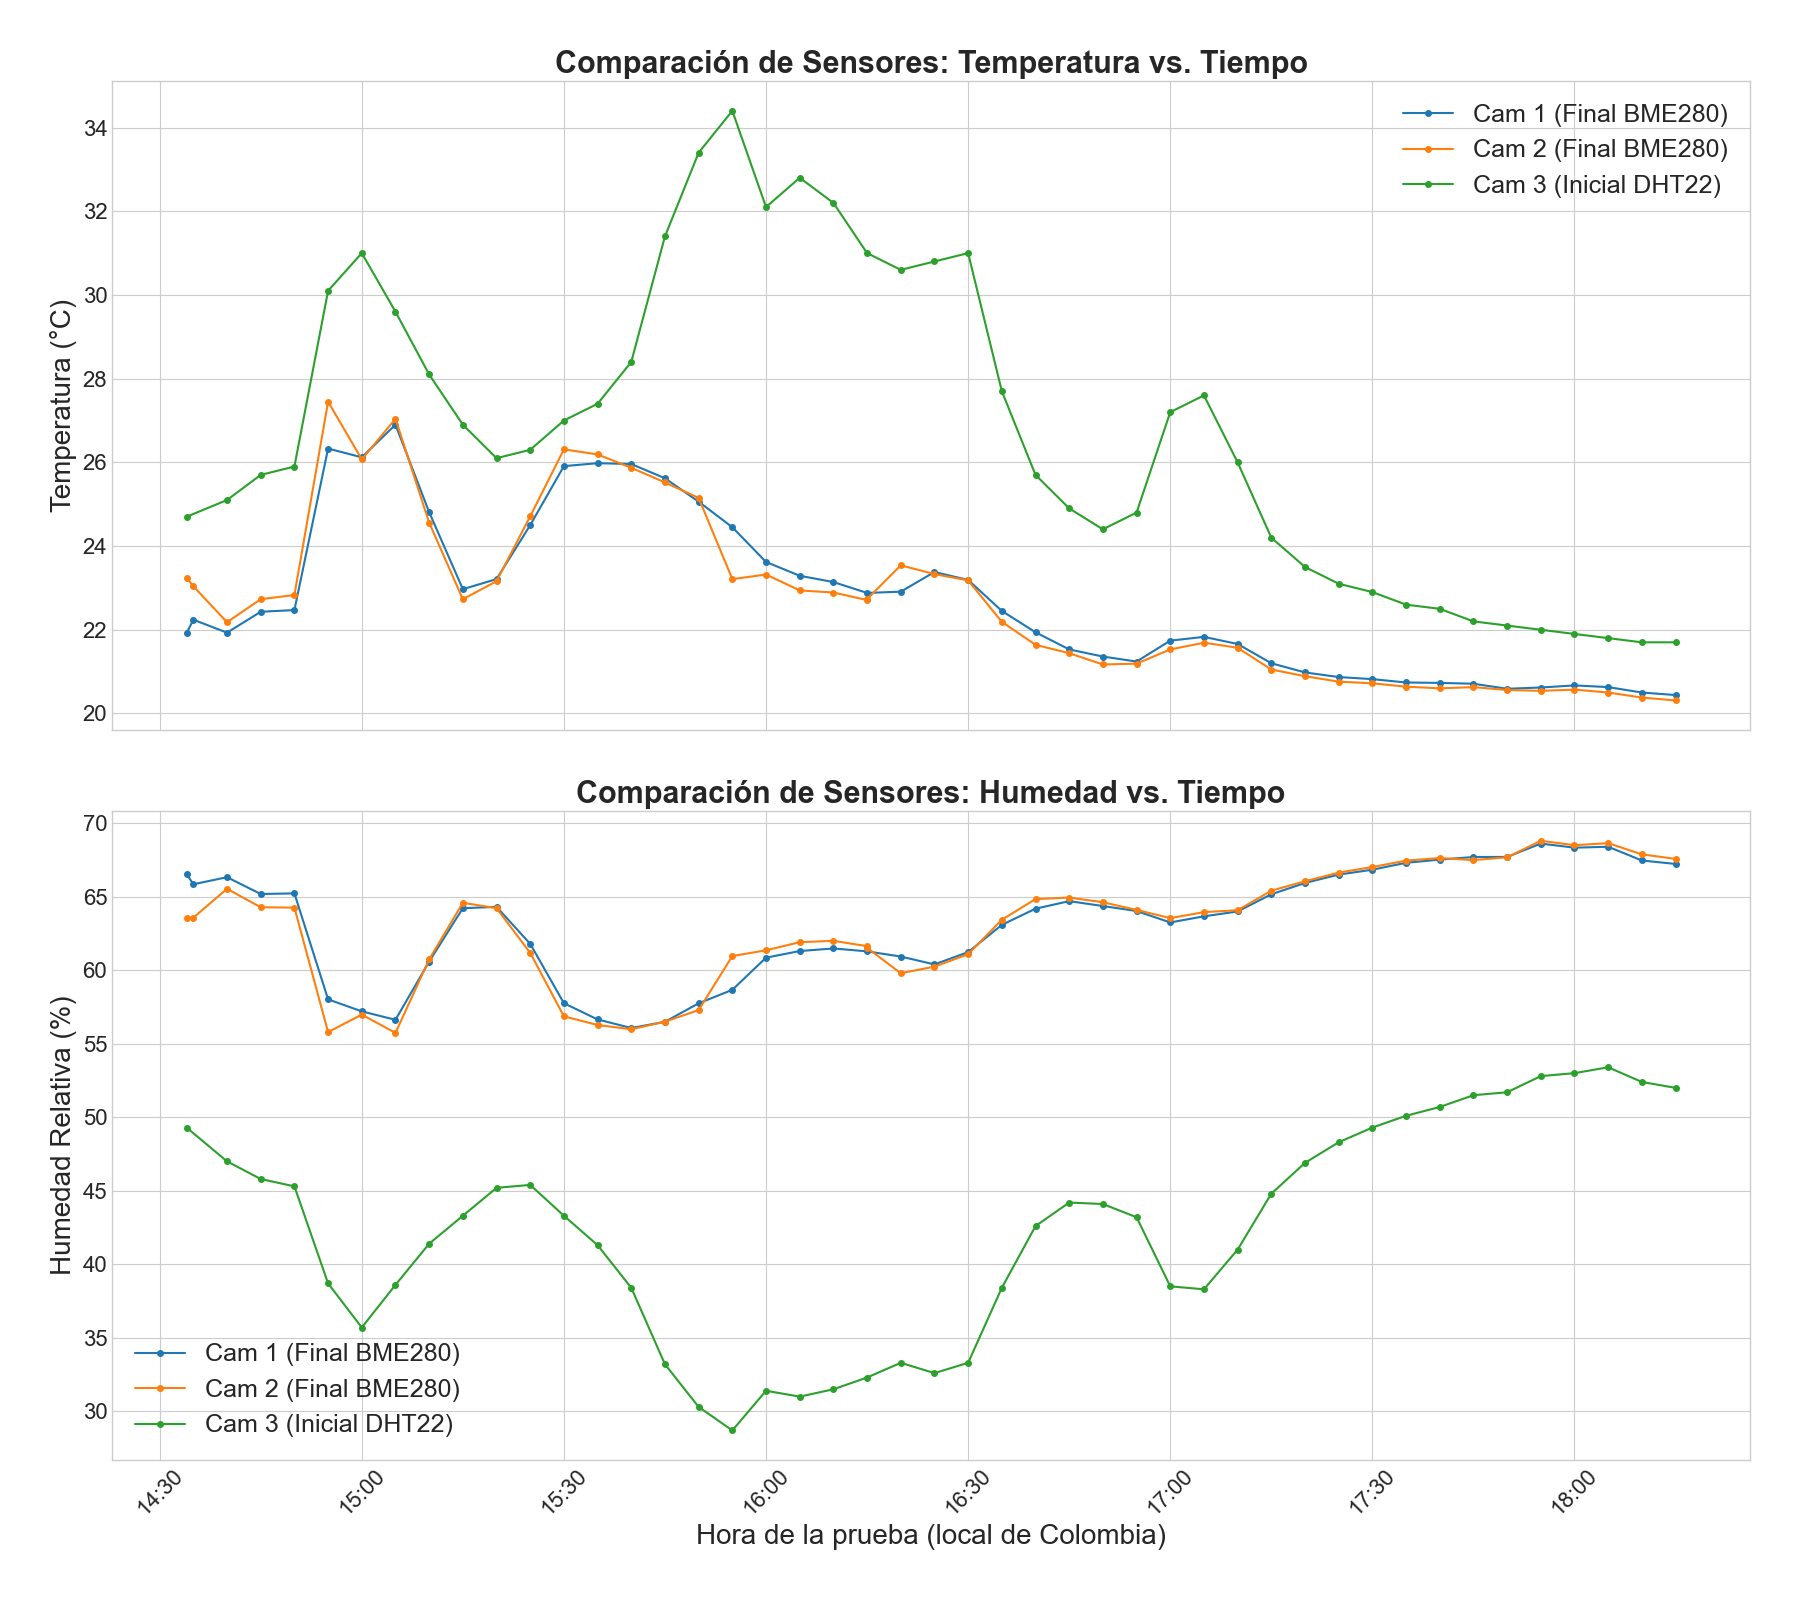
\includegraphics[width=\textwidth]{img/comparacion_ambiental.png}
    
    \vspace{0.2cm}
    \begin{minipage}{\textwidth}
    \small{\textit{Nota:} Desempeño de los sensores BME280 nuevos frente al sensor DHT22 usado.}
    \end{minipage}
    \label{fig:comparacion_ambiental}
\end{figure}

Profundizando en la sensibilidad ambiental, la Figura \ref{fig:contraste_ambiental} expone la prueba de contraste ambiental térmico sobre los sensores BME280. Al acercarles objetos con un gradiente térmico severo (vasos con hielo y agua hirviendo), todos los sensores reaccionaron de forma sinérgica, captando la perturbación térmica circundante de manera similar. Sin embargo, se evidenciaron variaciones minúsculas asociadas a la distancia geométrica relativa entre la fuente y cada sensor, así como perturbaciones (\textit{ruido}) introducidas por la disposición física del cableado en los protoboards, un factor clave a optimizar en la fase de diseño de la placa de circuito impreso (PCB).

\begin{figure}[H]
    \centering
    \caption{Contraste ambiental de temperatura y humedad.}
    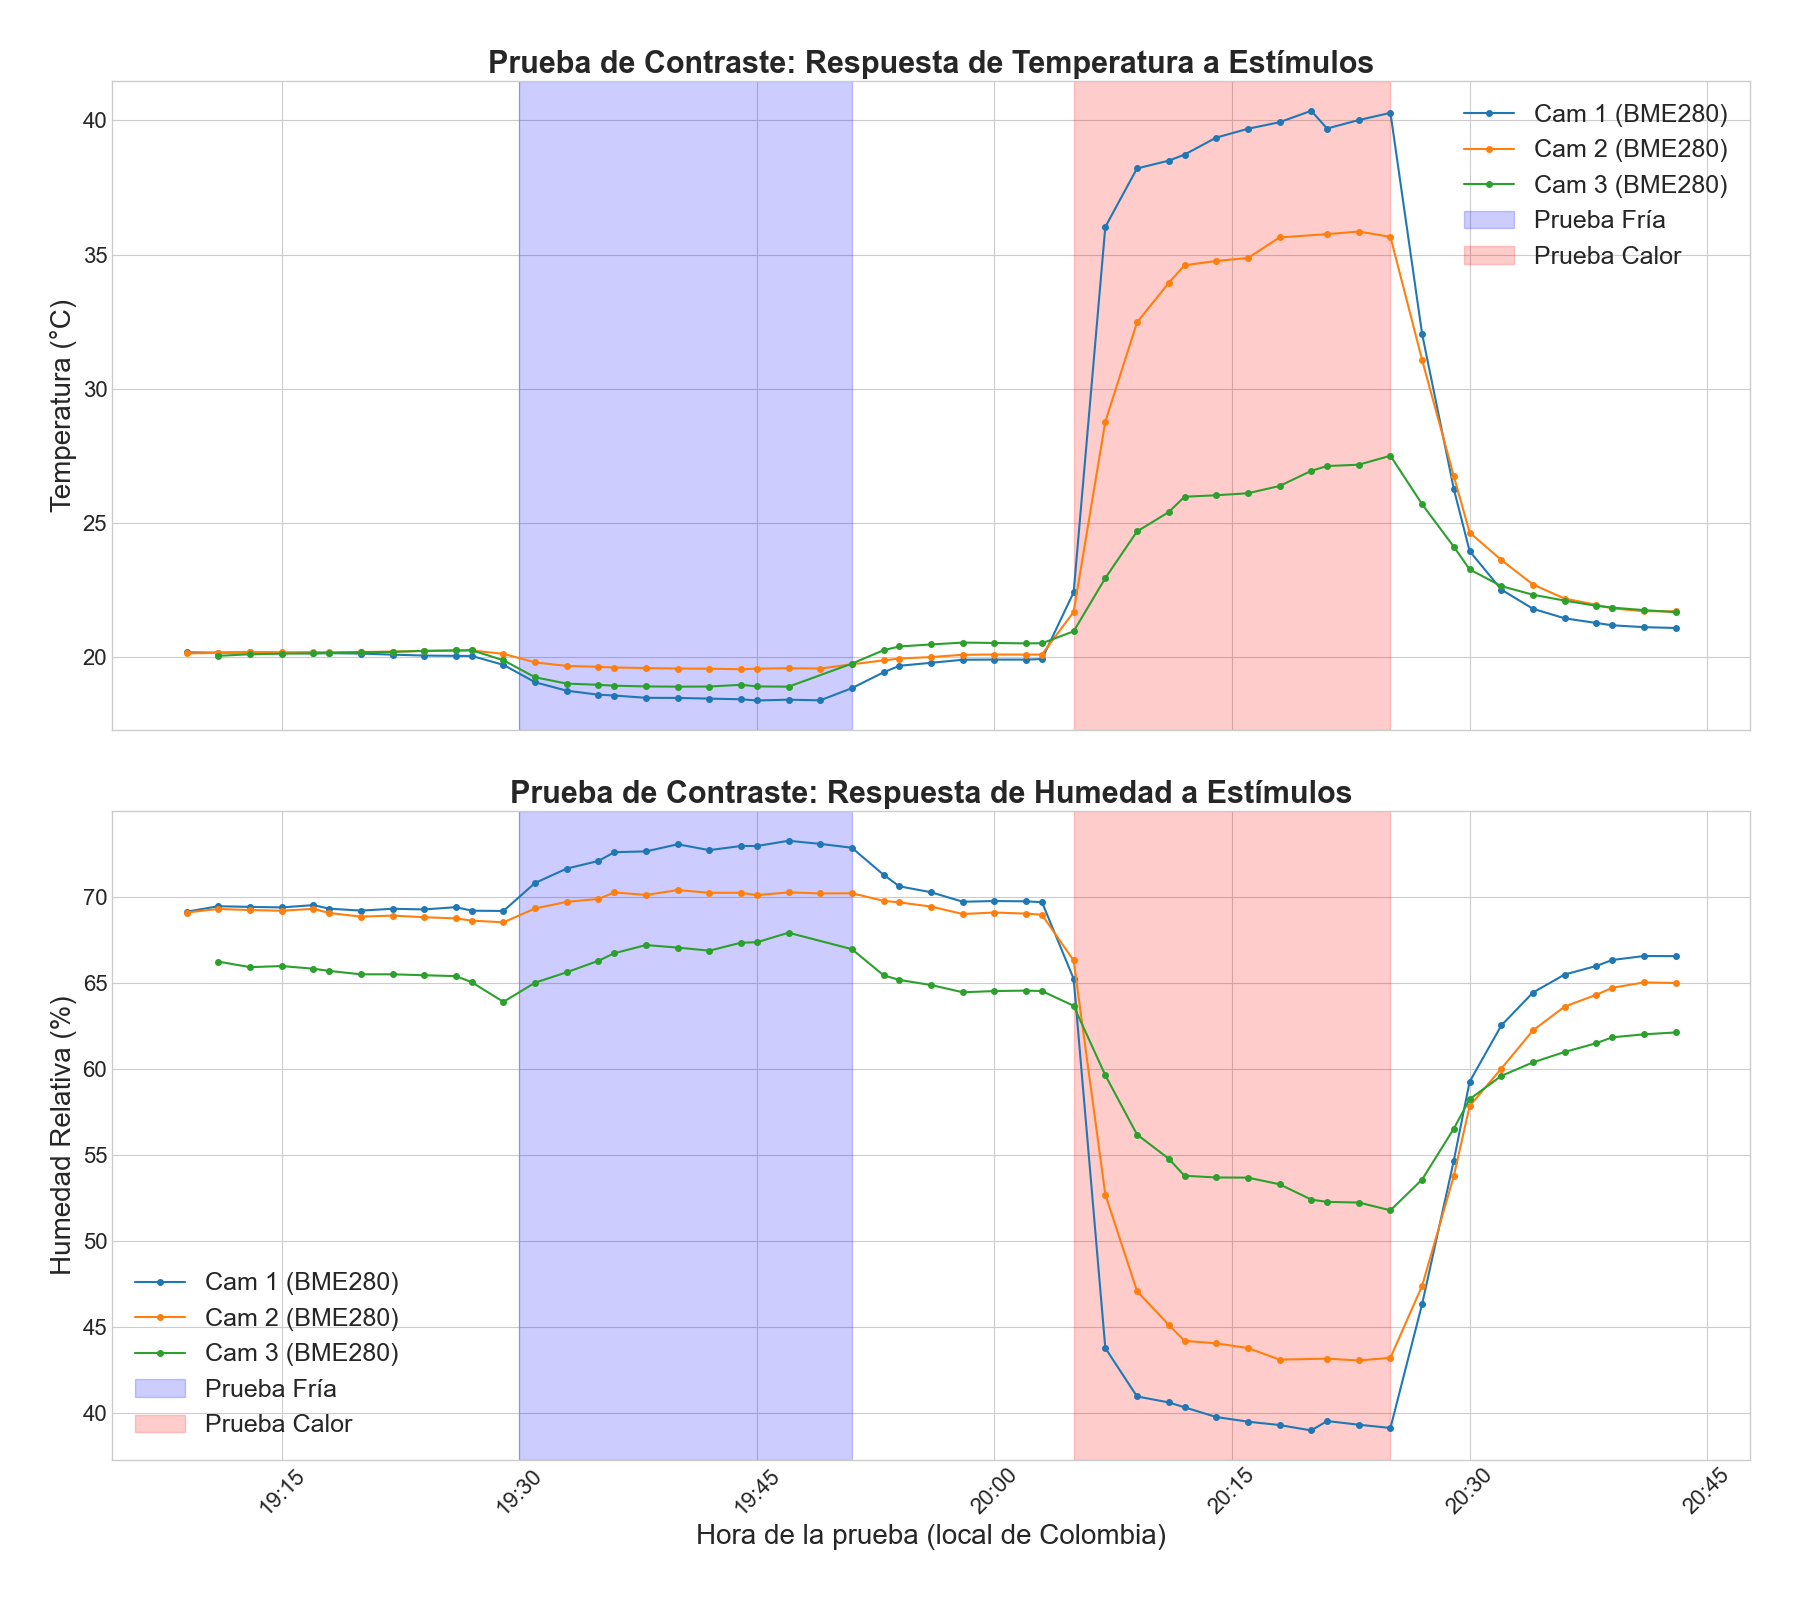
\includegraphics[width=\textwidth]{img/contraste_ambiental.png}
    
    \vspace{0.2cm}
    \begin{minipage}{\textwidth}
    \small{\textit{Nota:} Respuesta dinámica de los sensores BME280 ante elementos cálidos y fríos cercanos al encapsulado.}
    \end{minipage}
    \label{fig:contraste_ambiental}
\end{figure}

Finalmente, el registro de iluminancia a través de los fotorresistores BH1750 (Figura \ref{fig:comparacion_luminosidad}) corrobora el correcto funcionamiento del arreglo lumínico general. La diferencia entre las mediciones de los tres prototipos es marginal. Se observó, no obstante, una discreta presencia de ruido en las lecturas del sensor previamente utilizado, lo cual, aunque no invalida la medición, sugiere sutiles diferencias asociadas a la varianza de manufactura entre distintos encapsulados y fabricantes, o al propio desgaste de la fotorresistencia por uso continuo en campo.

\begin{figure}[H]
    \centering
    \caption{Medición comparativa de luminosidad ambiental.}
    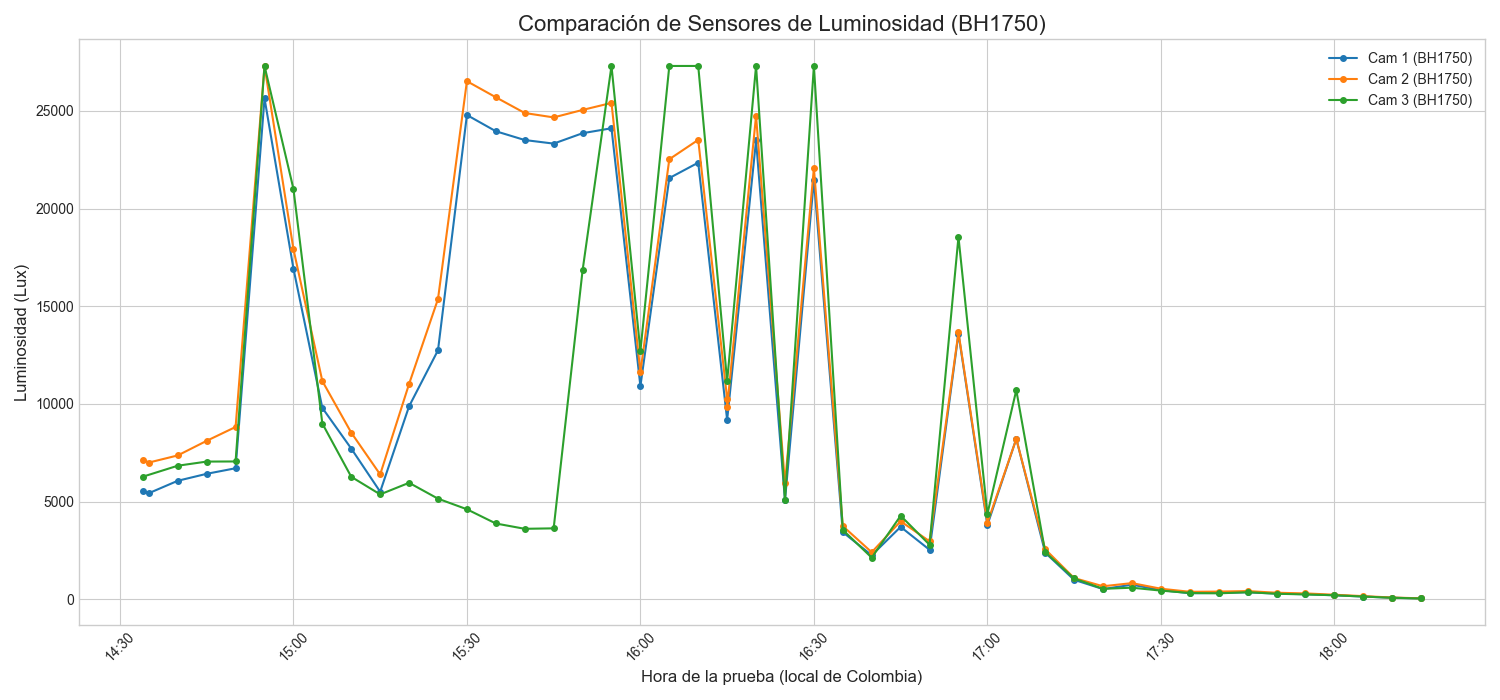
\includegraphics[width=\textwidth]{img/comparacion_luminosidad.png}
    
    \vspace{0.2cm}
    \begin{minipage}{\textwidth}
    \small{\textit{Nota:} Rendimiento y precisión de los sensores BH1750 instalados en las tres cámaras.}
    \end{minipage}
    \label{fig:comparacion_luminosidad}
\end{figure}

\subsection{Validación del sistema integrado}

\label{subsec:hardware_validacion_integrada}
La evaluación individual de los componentes clave proporciona la base para validar el desempeño del sistema de monitoreo termográfico en su conjunto. Los resultados presentados en las subsecciones anteriores (\ref{subsec:hardware_resultados_amb} y \ref{subsec:hardware_resultados_termico}) confirman la idoneidad de la arquitectura de hardware seleccionada para los prototipos finales (configuración de Cam 1 y Cam 2).

La combinación del microcontrolador ESP32-S3, el sensor ambiental microelectromecánico BME280 y los sensores térmicos MLX90640 (nuevos) demostró constituir un sistema de monitoreo estable y funcionalmente viable. Los sensores BME280 proporcionaron mediciones consistentes y fiables de temperatura y humedad ambiental, superando claramente al sensor DHT22 evaluado inicialmente. Los sensores térmicos MLX90640, cuando eran nuevos, mostraron una precisión aceptable para aplicaciones agrícolas, especialmente en rangos de temperatura cercanos a las condiciones ambientales y hasta 170°C (RMSE < 3,2°C). Aunque se observó un sesgo a temperaturas más elevadas (~190°C), este fue consistente y predecible, sugiriendo la posibilidad de corrección por software.

La integración física mediante protoboard y la conexión a través de las interfaces digitales estándar (I\textsuperscript{2}C para MLX90640, BME280, BH1750; DVP y SCCB/I\textsuperscript{2}C para OV2640; SPI para tarjeta SD) funcionaron según lo esperado, permitiendo al firmware desarrollado gestionar la adquisición de datos de todos los periféricos. Los componentes complementarios, como el sensor de luminosidad BH1750 y la cámara RGB OV2640, también operaron nominalmente, proveyendo el contexto ambiental y visual deseado. El regulador LM2596 suministró la alimentación de 3.3V de manera estable.

Un hallazgo fundamental de esta caracterización es la confirmación cuantitativa del impacto negativo del uso previo intensivo en la fiabilidad, particularmente evidente en el hardware del prototipo 3. Este resultado subraya la importancia crítica de utilizar componentes calibrados o al menos probados y verificar periódicamente su estado para asegurar la calidad de las mediciones en despliegues a largo plazo con tecnología de bajo costo.

Por lo que, la caracterización experimental valida que la arquitectura de hardware propuesta, implementada en los prototipos 1 y 2 con componentes seleccionados y probados, constituye un sistema integrado fiable y funcionalmente adecuado para la adquisición de datos termográficos y ambientales en el contexto agrícola. Esta validación es el fundamento técnico que permite posicionar al prototipo como una herramienta potencialmente útil y accesible para la monitorización del estrés hídrico y la toma de decisiones agronómicas.

Es importante realizar una aclaración metodológica respecto al despliegue posterior de estos prototipos validados. Si bien la electrónica y el software de los prototipos 1 y 2 demostraron un desempeño óptimo y simétrico durante la caracterización, su implementación inicial conjunta en un escenario comparativo multi-planta presentó desafíos a nivel de montaje físico. Como se detallará en el capítulo correspondiente al estudio experimental, el intento de operar múltiples dispositivos suspendidos mediante tensores introdujo una inestabilidad micromecánica que invalidó la captura de los termogramas. En consecuencia, aunque los protitpos 1 y2 fueron validados instrumentalmente con éxito en este capítulo, los datos recopilados por estos fueron descartados en la fase analítica final. Esto obligó a delimitar el alcance del proyecto hacia una Prueba de Concepto (PoC) estática de caso único o intracontrol ($n=1$), utilizando unicamente el prototipo 3 anclado de forma rígida, garantizando así la fiabilidad en la recolección de los datos agronómicos.

\subsection{Limitaciones y recomendaciones para trabajo futuro}
\label{subsec:hardware_limitaciones_futuro}
Si bien la caracterización realizada validó la funcionalidad básica y la viabilidad del prototipo de hardware, es importante reconocer las limitaciones inherentes a este estudio y proponer líneas de mejora y trabajo futuro centradas específicamente en el desarrollo del sistema físico.

Una limitación principal es que la validación del desempeño se realizó primordialmente en condiciones controladas (habitación cerrada y microinvernadero). Para consolidar la aplicabilidad real del sistema, es indispensable realizar evaluaciones exhaustivas a campo abierto. Esto expondrá el hardware a factores ambientales no controlados como la velocidad del viento (que puede afectar las lecturas de sensores de baja masa térmica \shortcite{GimenezGallego2021}), la lluvia, el polvo y la radiación solar directa, los cuales podrían impactar tanto la precisión de las mediciones como la durabilidad de los componentes. Podría ser necesario diseñar e implementar carcasas protectoras o filtros adicionales para mitigar estos efectos.

Asimismo, la calibración térmica, aunque efectiva para detectar inconsistencias y validar el rango operativo básico, se concentró en puntos de referencia a temperaturas relativamente altas o muy específicas. Futuros trabajos deberían incluir una caracterización más exhaustiva con puntos de referencia estables y precisos a lo largo de todo el espectro de temperaturas de interés agrícola (e.g., 10°C a 40°C), utilizando un sistema de calibración más exacto. Esto permitiría desarrollar modelos de corrección más robustos, posiblemente implementados directamente en el firmware, y realizar una calibración radiométrica más completa para mitigar la sensibilidad del sensor a influencias externas.

De cara al futuro, se proponen las siguientes mejoras y líneas de desarrollo para el hardware:
\begin{itemize}
    \item \textbf{Diseño modular y conectores:} El prototipado en protoboard, si bien útil para el desarrollo, no es robusto para despliegues a largo plazo. Se recomienda diseñar una placa de circuito impreso (PCB) a medida que integre los componentes principales. Además, implementar un sistema de conexión modular para los sensores (utilizando conectores estandarizados en lugar de conexiones directas o soldadas) facilitaría enormemente el reemplazo o la actualización de sensores individuales. Esto es particularmente relevante dado el impacto observado del desgaste en los componentes de bajo costo, permitiendo un mantenimiento más sencillo y económico.
    \item \textbf{Prototipos robustos y carcasas a medida:} Para mejorar la protección contra las condiciones ambientales de campo, se debe desarrollar una carcasa más robusta y específica para el dispositivo. El uso de impresión 3D permitiría diseñar e iterar rápidamente carcasas a medida que aseguren la protección de la electrónica, faciliten el montaje en campo (e.g., en postes o estructuras de soporte) y garanticen la exposición adecuada de los sensores al ambiente, minimizando al mismo tiempo la interferencia térmica de la propia carcasa.
    \item \textbf{Adaptación para plataformas móviles (drones):} Explorar la adaptación del diseño de hardware para su integración en vehículos aéreos no tripulados (UAVs o drones). Esto requeriría miniaturización adicional, optimización del consumo energético y posibles modificaciones en la óptica o el sistema de adquisición para mediciones aéreas, permitiendo cubrir áreas de cultivo más extensas.
    \item \textbf{Sistema de calibración mejorado:} Desarrollar un sistema de calibración de cuerpo negro más preciso y versátil que el utilizado en este estudio, capaz de generar y mantener temperaturas de referencia estables en un rango más amplio y relevante para la agricultura, y bajo diferentes condiciones de humedad y flujo de aire controlados.
\end{itemize}

La implementación de estas mejoras en el hardware contribuiría significativamente a aumentar la robustez, fiabilidad, facilidad de mantenimiento y aplicabilidad del sistema de monitoreo termográfico de bajo costo, acercándolo a una solución práctica y escalable para la agricultura de precisión.